%%%%%%%%%%%%%%%%%%%%%%%%%%%%%%%%%%%%%%%%%%%%%%%%%%%%%%%%%%%%%%%%%%%%%%%%%%%%%%%%
% TUM-Vorlage: Präsentation
%%%%%%%%%%%%%%%%%%%%%%%%%%%%%%%%%%%%%%%%%%%%%%%%%%%%%%%%%%%%%%%%%%%%%%%%%%%%%%%%
%
% Rechteinhaber:
%     Technische Universität München
%     https://www.tum.de
% 
% Gestaltung:
%     ediundsepp Gestaltungsgesellschaft, München
%     http://www.ediundsepp.de
% 
% Technische Umsetzung:
%     eWorks GmbH, Frankfurt am Main
%     http://www.eworks.de
%
%%%%%%%%%%%%%%%%%%%%%%%%%%%%%%%%%%%%%%%%%%%%%%%%%%%%%%%%%%%%%%%%%%%%%%%%%%%%%%%%


%%%%%%%%%%%%%%%%%%%%%%%%%%%%%%%%%%%%%%%%%%%%%%%%%%%%%%%%%%%%%%%%%%%%%%%%%%%%%%%%
% Zur Wahl des Seitenverhältnisses bitte einen der beiden folgenden Befehle
% auskommentieren und den ausführen lassen:
\documentclass[t]{beamer}
\usepackage[
    orientation=landscape,
    size=custom,
    width=25.4,
    height=19.05,
    scale=0.63 % erzeugt 16pt Schriftgröße
]{beamerposter}

\newcommand{\PraesentationSchriftgroesseSehrGross}{\fontsize{30}{45}}
\newcommand{\PraesentationSchriftgroesseGross}{\fontsize{22}{33}}
\newcommand{\PraesentationSchriftgroesseNormal}{\fontsize{16}{29}}
\newcommand{\PraesentationSchriftgroesseKlein}{\fontsize{12}{18}}
\newcommand{\PraesentationSchriftgroesseDreizeiler}{\fontsize{7}{10}}
\newcommand{\PraesentationSchriftgroesseAufzaehlungszeichen}{\fontsize{10}{8}}

\newcommand{\PraesentationAbstandAbsatz}{22.1pt}
\newcommand{\PraesentationPositionKorrekturOben}{0cm}
\newcommand{\PraesentationBeispieleSchriftgroessen}{30 | 22 | 16 | 12}
\usepackage[utf8]{inputenc}
\usepackage[T1]{fontenc} % Zeichensatzkodierung

\usepackage{calc} % Berechnungen

\usepackage[english]{babel} % Deutsche Lokalisierung
\usepackage{graphicx} % Grafiken
\usepackage[absolute, overlay]{textpos} % Positionierung

% Silbentrennung:
\usepackage{hyphenat}
%\tolerance 2414
%\hbadness 2414
%\emergencystretch 1.5em
%\hfuzz 0.3pt
%\widowpenalty=10000     % Hurenkinder
%\clubpenalty=10000      % Schusterjungen
%\vfuzz \hfuzz

% Euro-Symbol:
\usepackage[gen]{eurosym}
\DeclareUnicodeCharacter{20AC}{\euro{}}

% Schriftart Helvetica:
\usepackage[scaled]{helvet}
\usefonttheme[onlymath]{serif}
\renewcommand{\familydefault}{\sfdefault}

\usepackage{mathptmx} % skalierbare Formelschriften

\usepackage{tabularx}

\usepackage{multicol} % mehrspaltiger Text

\usepackage{tikz}
\usetikzlibrary{arrows, shapes, shapes.multipart, trees, positioning,
    backgrounds, fit, matrix, external}

% Diagramme:
\usepackage{pgfplots}
\pgfplotsset{compat=default}

% Erweiterbare Fusszeile:
\newcommand{\PraesentationFusszeileZusatz}{}

\usepackage{bookmark} % Lesezeichen
\usepackage{multirow}
\usepackage{siunitx}
\usepackage{caption}
\usepackage{subcaption}
\usepackage[export]{adjustbox}
\usepackage{array}
\usepackage{amsmath,verbatim,float,caption,subcaption}
\usepackage{mathtools}
\usepackage[style=ieee]{biblatex}
\addbibresource{Literature.bib}
\setbeamertemplate{bibliography item}{\insertbiblabel}
\DeclareMathOperator{\arctanh}{arctanh}
\DeclarePairedDelimiter\abs{\lvert}{\rvert}
\graphicspath{{../Figures/}, {../Figures/pdf/}, {..//Figures/png/}, {../Figures/pdf/loop/}, {../Figures/pdf/patch/}, {../Figures/pdf/resistor/}, 
	{../Figures/pdf/bpf/}, {../Figures/pdf/bpfs/}, {../Figures/pdf/wilkinson/}}
\renewcommand{\Re}{\operatorname{Re}}
\renewcommand{\Im}{\operatorname{Im}}

% Unterdrückung layoutbedingter Warnungen
\usepackage[immediate]{silence}
\WarningFilter[layout]{lastpage}{Rerun to get the references right} % Gesamtseitenzahl
\WarningFilter[layout]{latex}{Label(s) may have changed.} % Referenz auf letzte Seite
\WarningFilter[layout]{pgfplots}{running in backwards compatibility mode (unsuitable tick labels; missing features).} % Labelerstellung ab Version 1.17 nicht abwärtskompatibel
\WarningFilter[layout]{latex}{There were undefined references}
\WarningFilter[layout]{latex}{Reference `PraesentationDiagramm} % Erstellung einer Legende außerhalb des Diagrammbereichs

% Debugging:
%\DeactivateWarningFilters[layout] % Unterdrückte Warnungen einschalten % Seitenverhältnis 4:3
% \input{./Ressourcen/Praesentation/Praeambel16zu9.tex} % Seitenverhältnis 16:9
%%%%%%%%%%%%%%%%%%%%%%%%%%%%%%%%%%%%%%%%%%%%%%%%%%%%%%%%%%%%%%%%%%%%%%%%%%%%%%%%


%%%%%%%%%%%%%%%%%%%%%%%%%%%%%%%%%%%%%%%%%%%%%%%%%%%%%%%%%%%%%%%%%%%%%%%%%%%%%%%%
%%%%%%%%%%%%%%%%%%%%%%%%%%%%%%%%%%%%%%%%%%%%%%%%%%%%%%%%%%%%%%%%%%%%%%%%%%%%%%%%
% TUM-Vorlage: Personenspezifische Informationen
%%%%%%%%%%%%%%%%%%%%%%%%%%%%%%%%%%%%%%%%%%%%%%%%%%%%%%%%%%%%%%%%%%%%%%%%%%%%%%%%
%
% Rechteinhaber:
%     Technische Universität München
%     https://www.tum.de
% 
% Gestaltung:
%     ediundsepp Gestaltungsgesellschaft, München
%     http://www.ediundsepp.de
% 
% Technische Umsetzung:
%     eWorks GmbH, Frankfurt am Main
%     http://www.eworks.de
%
%%%%%%%%%%%%%%%%%%%%%%%%%%%%%%%%%%%%%%%%%%%%%%%%%%%%%%%%%%%%%%%%%%%%%%%%%%%%%%%%

% Für die Person anpassen:

\newcommand{\PersonTitel}{}
\newcommand{\PersonVorname}{Berke}
\newcommand{\PersonNachname}{Karakin}
\newcommand{\PersonStadt}{@Ort@}
\newcommand{\PersonAdresse}{%
    @Adresse@\\%
    @Plz@~\PersonStadt%
}
\newcommand{\PersonTelefon}{@Telefon@}
\newcommand{\PersonFax}{@Fax@}
\newcommand{\PersonEmail}{@E-Mail@}
\newcommand{\PersonWebseite}{@Web@}

\newcommand{\FakultaetAnsprechpartner}{@Ansprechpartner@}
\newcommand{\LehrstuhlName}{Chair of High-Frequency Engineering}

\hyphenation{} % eigene Silbentrennung                    % !!! DATEI ANPASSEN !!!
%%%%%%%%%%%%%%%%%%%%%%%%%%%%%%%%%%%%%%%%%%%%%%%%%%%%%%%%%%%%%%%%%%%%%%%%%%%%%%%%


\renewcommand{\PersonTitel}{}
\newcommand{\Datum}{\today}

\renewcommand{\PraesentationFusszeileZusatz}{}

\title{Designing Test Targets for Verification of an Inverse Source Solver at Low Frequencies}
\author{\PersonTitel{} \PersonVorname{} \PersonNachname}
\institute[]{\UniversitaetName \\ \FakultaetName \\ \LehrstuhlName}
\date[\Datum]{Munich, July 1, 2024}
\subject{}


%%%%%%%%%%%%%%%%%%%%%%%%%%%%%%%%%%%%%%%%%%%%%%%%%%%%%%%%%%%%%%%%%%%%%%%%%%%%%%%%
%%%%%%%%%%%%%%%%%%%%%%%%%%%%%%%%%%%%%%%%%%%%%%%%%%%%%%%%%%%%%%%%%%%%%%%%%%%%%%%%
% EINSTELLUNGEN
%%%%%%%%%%%%%%%%%%%%%%%%%%%%%%%%%%%%%%%%%%%%%%%%%%%%%%%%%%%%%%%%%%%%%%%%%%%%%%%%

% Allgemein:
\newcommand{\AllgemeinGestalter}{ediundsepp Gestaltungsgesellschaft}
\newcommand{\AllgemeinErsteller}{eWorks GmbH}

% Universität:
\newcommand{\UniversitaetName}{Technical University of Munich}
\newcommand{\UniversitaetAbkuerzung}{TUM}
\newcommand{\UniversitaetWebseite}{www.tum.de}
\newcommand{\UniversitaetLogoBreite}{19mm}
\newcommand{\UniversitaetLogoHoehe}{1cm}

\newcommand{\UniversitaetAdresse}{%
    Arcisstraße~21\\%
    80333~München%
}

% Fakultät:
\newcommand{\FakultaetName}{TUM School of Computation, Information and Technology}



\newcommand{\PraesentationSeitenrand}{8.9mm}
\newcommand\crule[3][black]{\textcolor{#1}{\rule{#2}{#3}}}

\newlength\smallerbaselineskip
\setlength{\smallerbaselineskip}{0.8\baselineskip}

    % Blautöne:
\definecolor{TUMBlau}{RGB}{0,101,189} % Pantone 300
\definecolor{TUMBlauDunkel}{RGB}{0,82,147} % Pantone 301
\definecolor{TUMBlauHell}{RGB}{152,198,234} % Pantone 283
\definecolor{TUMBlauMittel}{RGB}{100,160,200} % Pantone 542

    % Hervorhebung:
\definecolor{TUMElfenbein}{RGB}{218,215,203} % Pantone 7527 -Elfenbein
\definecolor{TUMGruen}{RGB}{162,173,0} % Pantone 383 - Grün
\definecolor{TUMOrange}{RGB}{227,114,34} % Pantone 158 - Orange
\definecolor{TUMGrau}{gray}{0.6} % Grau 60%


\setbeamercolor*{alerted text}{fg=TUMOrange}

\newcommand{\PraesentationSetzeTextfarbe}{
    \color{PraesentationTextfarbe}
    \setbeamercolor*{frametitle}{fg=PraesentationTextfarbe}
    \setbeamercolor*{normal text}{fg=PraesentationTextfarbe}
    \setbeamercolor{itemize/enumerate body}{fg=PraesentationTextfarbe}
    \setbeamercolor*{itemize item}{fg=PraesentationTextfarbe}
}

\newcommand{\PraesentationFarbschemaStandard}{
    \setbeamercolor*{background canvas}{}
    \definecolor{PraesentationTextfarbe}{rgb}{0,0,0}
    \PraesentationSetzeTextfarbe
}

\newcommand{\PraesentationFarbschemaWeissBlau}{
    \setbeamercolor*{background canvas}{bg=TUMBlauDunkel}
    \definecolor{PraesentationTextfarbe}{rgb}{1,1,1}
    \PraesentationSetzeTextfarbe
}

\newcommand{\PraesentationFarbschemaWeissSchwarz}{
    \setbeamercolor*{background canvas}{bg=black}
    \definecolor{PraesentationTextfarbe}{rgb}{1,1,1}
    \PraesentationSetzeTextfarbe
}

\newcommand{\PraesentationTitelseiteInhalt}{
    \begin{textblock*}{\paperwidth}[0,0](0cm,-\PraesentationSeitenrand + 10mm + \PraesentationPositionKorrekturOben)%
        \color{PraesentationTextfarbe}%
        \frametitle{\inserttitle}
        \vspace*{49.4mm}
        \usebeamerfont{author}\selectfont\insertauthor\\
        \insertinstitute\\
        \insertdate%
    \end{textblock*}
}

\newcommand{\PraesentationSeitenkopfInhalt}[1]{
    %\vspace*{31.7mm}%
    \begin{textblock*}{1.68cm}[1,0](\paperwidth - \PraesentationSeitenrand - \PraesentationSeitenrand, 0cm)%
        \includegraphics[width=1.68cm]{#1}%
    \end{textblock*}
    \begin{textblock*}{3cm}[1,0](\paperwidth - \PraesentationSeitenrand, -\PraesentationSeitenrand)%
        \hbox{%
            \color{PraesentationTextfarbe}
            \hbox{\insertframenavigationsymbol}%
            \hbox{\insertsubsectionnavigationsymbol}%
            \hbox{\insertsectionnavigationsymbol}%
        }%
    \end{textblock*}%
}

\newcommand{\PraesentationBildUhrenturm}{%
    \begin{textblock*}{10.82cm}[1,1](\paperwidth - \PraesentationSeitenrand - \PraesentationSeitenrand, \paperheight - 9mm)%
        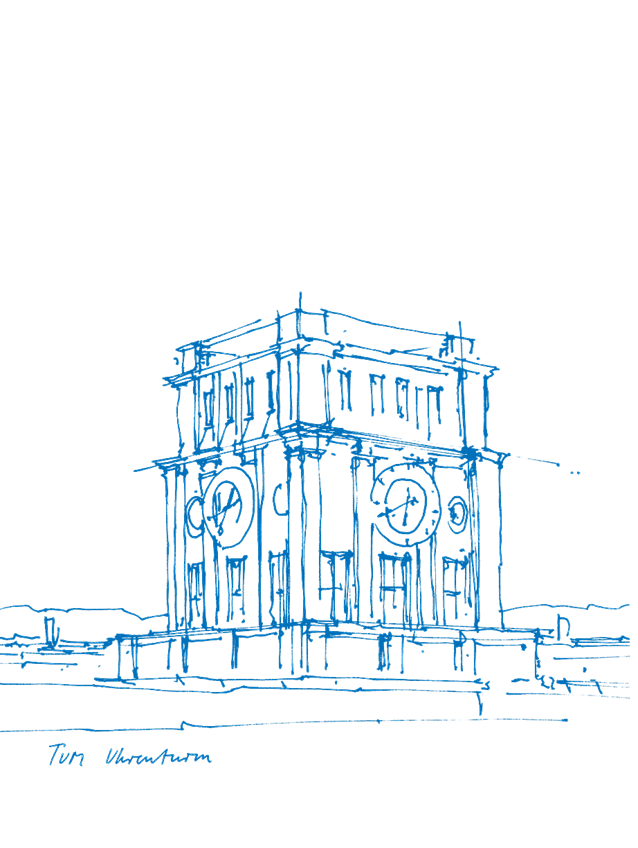
\includegraphics{./Ressourcen/Praesentation/Bilder/TUM_Uhrenturm.png}%
    \end{textblock*}%
}

\newcommand{\PraesentationStartseiteUhrenturm}{
    \setbeamertemplate{title page}{%
        \PraesentationSeitenkopfInhalt{./Ressourcen/_Bilder/Universitaet_Logo_RGB.pdf}
        \PraesentationBildUhrenturm
        \PraesentationTitelseiteInhalt
    }
}

\newcommand{\PraesentationStartseiteFlaggen}{
    \setbeamertemplate{title page}{%
        \begin{textblock*}{\paperwidth}[0,1](-\PraesentationSeitenrand,\paperheight-\PraesentationSeitenrand)%
            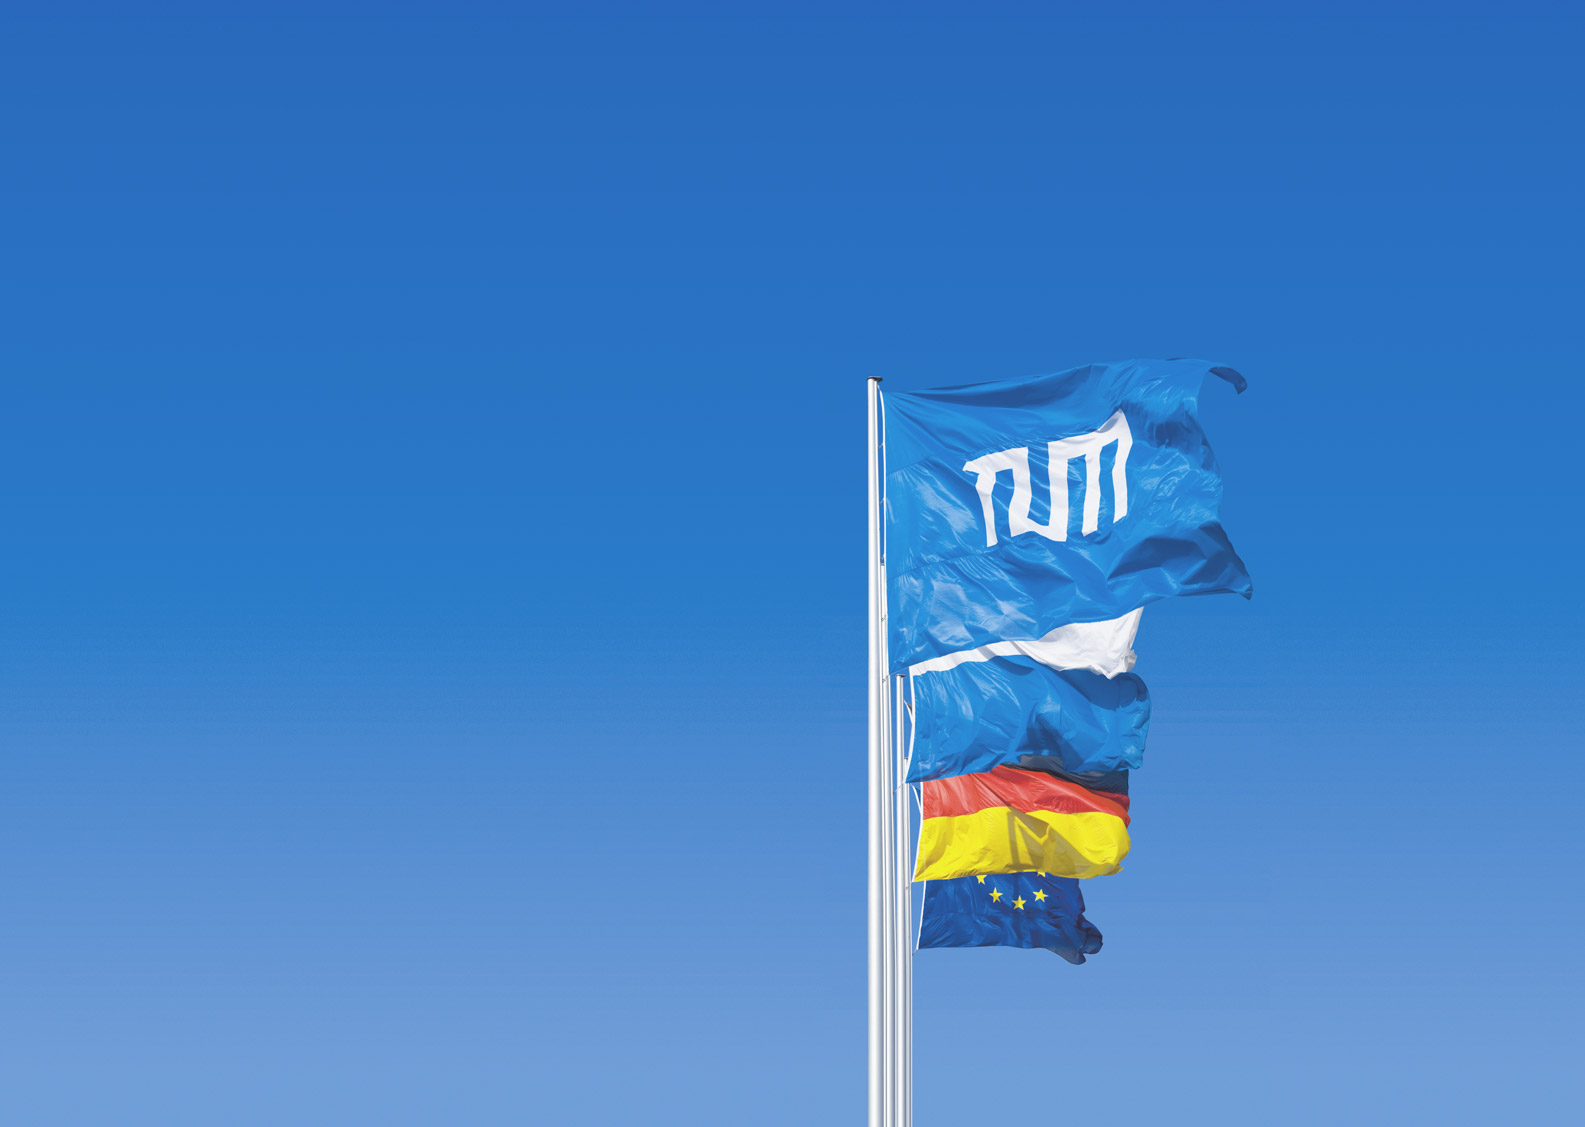
\includegraphics[width=\paperwidth]{./Ressourcen/Praesentation/Bilder/Universitaet_Flaggen.jpg}%
        \end{textblock*}
        \PraesentationSeitenkopfInhalt{./Ressourcen/_Bilder/Universitaet_Logo_weiss.pdf}
        \PraesentationTitelseiteInhalt
    }
}

\newcommand{\PraesentationStartseiteLeer}{
    \setbeamertemplate{title page}{%
        \PraesentationSeitenkopfInhalt{./Ressourcen/_Bilder/Universitaet_Logo_weiss.pdf}
        \PraesentationTitelseiteInhalt
    }
}


\newcommand{\PraesentationMasterStandard}{
    \PraesentationFarbschemaStandard

    \PraesentationStartseiteUhrenturm

    \setbeamertemplate{headline}{
        \PraesentationSeitenkopfInhalt{./Ressourcen/_Bilder/Universitaet_Logo_RGB.pdf}
    }
}

\newcommand{\PraesentationMasterWeissBlau}{
    \PraesentationFarbschemaWeissBlau

    \PraesentationStartseiteLeer

    \setbeamertemplate{headline}{
        \PraesentationSeitenkopfInhalt{./Ressourcen/_Bilder/Universitaet_Logo_weiss.pdf}
    }
}

\newcommand{\PraesentationMasterKopfzeileDreizeiler}{
    \PraesentationFarbschemaStandard

    \setbeamertemplate{title page}{%
        \PraesentationBildUhrenturm
        \begin{textblock*}{\paperwidth}[0,0](0cm, -7.8mm)%
            \color{TUMBlau}\PraesentationSchriftgroesseDreizeiler\selectfont%
            \LehrstuhlName\\%
            \FakultaetName\\%
            \UniversitaetName\\%
            \normalcolor\normalsize\selectfont%
        \end{textblock*}%
        \PraesentationSeitenkopfInhalt{./Ressourcen/_Bilder/Universitaet_Logo_RGB.pdf}
        \PraesentationTitelseiteInhalt
    }
}

\newcommand{\PraesentationMasterWeissSchwarz}{
    \PraesentationFarbschemaWeissSchwarz

    \setbeamertemplate{title page}{%
        \PraesentationTitelseiteInhalt
        \PraesentationSeitenkopfInhalt{./Ressourcen/_Bilder/Universitaet_Logo_weiss.pdf}
    }

    \setbeamertemplate{headline}{
        \PraesentationSeitenkopfInhalt{./Ressourcen/_Bilder/Universitaet_Logo_weiss.pdf}
    }
}

\newcommand{\PraesentationTitelseite}{\frame[plain]{\titlepage}}
\newcommand{\PraesentationUeberschriftZweizeilig}[2]{\frametitle{#1\\[5mm]#2}}

\setbeamersize{
    text margin left=\PraesentationSeitenrand,
    text margin right=\PraesentationSeitenrand
}

\setbeamertemplate{frametitle}{%
    {\rule{0pt}{42mm + \PraesentationPositionKorrekturOben}\PraesentationSchriftgroesseSehrGross\selectfont\insertframetitle\newline\vspace*{-6.7mm}}%
}

% Aufzählungen:
\newcommand{\PraesentationAufzaehlungEbeneEinsSymbol}{\raise2pt\hbox{\donotcoloroutermaths\usebeamercolor{itemize subitem}\PraesentationSchriftgroesseAufzaehlungszeichen$\bullet$}}
\newcommand{\PraesentationAufzaehlungEbeneZweiSymbol}{\raise1.25pt\hbox{\donotcoloroutermaths\usebeamercolor{itemize subitem}$-$}}
\setbeamertemplate{itemize items}[circle]
\setbeamertemplate{itemize subitem}[triangle]
\setbeamercolor{itemize subitem}{fg=black}
\setbeamerfont{itemize/enumerate subbody}{size=\normalsize}
\setbeamertemplate{itemize item}{\PraesentationAufzaehlungEbeneEinsSymbol}
\setbeamertemplate{itemize subitem}{\PraesentationAufzaehlungEbeneZweiSymbol{}}
%\addtolength{\leftmarginii}{16mm-2pt}%

\newenvironment{PraesentationAufzaehlung}
{%
    \vspace{-\baselineskip}%
    \begin{itemize}%
        \setlength{\itemsep}{0pt}%
        \setlength{\parskip}{0pt}%
        \setlength{\parsep}{0pt}%
        \addtolength{\itemindent}{-1ex}%
}{%
    \end{itemize}%
}

%%%%%%%%%%%%%%%%%%%%%%%%%%%%%%%%%%%%%%%%%%%%%%%%%%%%%%%%%%%%%%%%%%%%%%%%%%%%%%%%
% DOKUMENT
%%%%%%%%%%%%%%%%%%%%%%%%%%%%%%%%%%%%%%%%%%%%%%%%%%%%%%%%%%%%%%%%%%%%%%%%%%%%%%%%


% PDF-Einstellungen:
\hypersetup{
    pdfstartview={Fit},
    pdfproducer={\AllgemeinErsteller},
    pdfcreator={\AllgemeinGestalter}
}

\setbeamercolor{bibliography item}{fg=black}
\setbeamercolor{bibliography entry author}{fg=black}
\setbeamercolor{bibliography entry title}{fg=black}
\setbeamercolor{bibliography entry location}{fg=black}
\setbeamercolor{bibliography entry note}{fg=black}

\textblockorigin{\PraesentationSeitenrand}{\PraesentationSeitenrand} % Ursprung für Positionierung

\setbeamerfont{footnote}{size=\PraesentationSchriftgroesseKlein}

\setbeamertemplate{footline}{
    \hbox{%
        %\usebeamerfont{footnote}%
        \begin{beamercolorbox}[wd=.9\paperwidth]{}%
            \hspace*{\PraesentationSeitenrand}%
            \PersonTitel{} ~~ \PraesentationFusszeileZusatz{}%
        \end{beamercolorbox}%
        \begin{beamercolorbox}[wd=.1\paperwidth]{}%
            \insertframenumber{}%
            \raggedleft
            \hspace*{\PraesentationSeitenrand}%
        \end{beamercolorbox}%
        \vspace*{3.25mm}%
    }%
}

\setbeamertemplate{navigation symbols}{}
\setbeamercolor*{caption name}{fg = TUMBlau}
    
\begin{document}
\setlength{\baselineskip}{\PraesentationAbstandAbsatz}
\setlength{\parskip}{\baselineskip}

 % !!! NICHT ENTFERNEN !!!
%%%%%%%%%%%%%%%%%%%%%%%%%%%%%%%%%%%%%%%%%%%%%%%%%%%%%%%%%%%%%%%%%%%%%%%%%%%%%%%%


%%%%%%%%%%%%%%%%%%%%%%%%%%%%%%%%%%%%%%%%%%%%%%%%%%%%%%%%%%%%%%%%%%%%%%%%%%%%%%%%
% FOLIENSTIL: Standard
\PraesentationMasterStandard

\PraesentationMasterKopfzeileDreizeiler
\PraesentationTitelseite % Fügt die Startseite ein


%%%%%%%%%%%%%%%%%%%%%%%%%%%%%%%%%%%%%%%%%%%%%%%%%%%%%
%% Beispielfolien                                  %%
%%%%%%%%%%%%%%%%%%%%%%%%%%%%%%%%%%%%%%%%%%%%%%%%%%%%%%%%%%%%%%%%%%%%%%%%%%%%%%%%%
% TUM-Vorlage: Präsentation - Beispiele
%%%%%%%%%%%%%%%%%%%%%%%%%%%%%%%%%%%%%%%%%%%%%%%%%%%%%%%%%%%%%%%%%%%%%%%%%%%%%%%%


%%%%%%%%%%%%%%%%%%%%%%%%%%%%%%%%%%%%%%%%%%%%%%%%%%%%%
%% Folie: Gültigkeit der Masterfolien              %%
%%%%%%%%%%%%%%%%%%%%%%%%%%%%%%%%%%%%%%%%%%%%%%%%%%%%%

\begin{frame}
    \frametitle{Gültigkeit der Masterfolien}

Dieser Folienmaster gilt bei offiziellen Präsentationen im Rahmen der TUM. Es
ist darauf zu achten, dass wir uns in einem durchgängigen Layout präsentieren.

Abweichungen vom vorgegebenen Layout bitte auf ein Minimum reduzieren.

\end{frame}
\clearpage


%%%%%%%%%%%%%%%%%%%%%%%%%%%%%%%%%%%%%%%%%%%%%%%%%%%%%
%% Folie: Grundlage der Masterfolien               %%
%%%%%%%%%%%%%%%%%%%%%%%%%%%%%%%%%%%%%%%%%%%%%%%%%%%%%

\begin{frame}
    \frametitle{Grundlage der Masterfolien}

Als Grundlage dient der Corporate Design Style Guide der TUM.\newline
Die Präsentationsvorlage ist auf gute Lesbarkeit und klare Darstellung von
Informationen optimiert.

\end{frame}
\clearpage


%%%%%%%%%%%%%%%%%%%%%%%%%%%%%%%%%%%%%%%%%%%%%%%%%%%%%
%% Folie: 2-zeilige Überschrift                    %%
%%%%%%%%%%%%%%%%%%%%%%%%%%%%%%%%%%%%%%%%%%%%%%%%%%%%%

\begin{frame}
    \PraesentationUeberschriftZweizeilig{Hier steht eine}{2-zeilige Überschrift}

Als Grundlage dient der Corporate Design Style Guide der TUM.\newline
Die Präsentationsvorlage ist auf gute Lesbarkeit und klare Darstellung von
Informationen optimiert.

\end{frame}
\clearpage


%%%%%%%%%%%%%%%%%%%%
%% Folie: Schrift %%
%%%%%%%%%%%%%%%%%%%%
\begin{frame}
    \frametitle{Schrift}

Das Grundprinzip ist, Informationen bestmöglich zu transportieren. Dazu muss
vor allem die Schrift einheitlich und für alle im Raum lesbar sein.

Schriftart: Helvetica

Schriftgößen: \PraesentationBeispieleSchriftgroessen

Zeilenabstand: 1,15 mm

Die Einstellungen sind für diese Vorlage als Standard eingestellt. Bei
Diagrammen und Tabellen muss die Schriftgröße ggf. angepasst werden. Für
Ausszeichnungen im Fließtext kann auch \textbf{fett} markiert werden. Bei
großer Distanz bzw. kleinem Präsenationsmedium kann der Schriftgrad notfalls
proportional erhöht werden.

\end{frame}
\clearpage


%%%%%%%%%%%%%%%%%%%
%% Folie: Farben %%
%%%%%%%%%%%%%%%%%%%
\begin{frame}
    \frametitle{Farben}
    
Als erstes soll mit schwarz und weiß gearbeitet werden.\newline
Für Aufwändigere Darstellungen sind Farben mit Bedacht und in möglichst
geringem Umfang einzusetzen.

In diesem Folienmaster ist die Farbpalette festgelegt.

{
    \renewcommand{\arraystretch}{1.2} % skaliert die Tabellen mit Farbfeldern

    Zuerst mit den Primärfarben arbeiten.

    \setlength{\fboxsep}{-1pt} \setlength{\fboxrule}{1pt} % fbox/framebox konfigurieren

    \vspace*{-5mm}
   \begin{tabular}{@{}lll}
        \crule[TUMBlau]{24mm}{6mm}
        & \crule[black]{24mm}{6mm}
        & \fbox{\crule[white]{24mm}{6mm}}
    \end{tabular}

    \vspace*{-5mm}
    Für z.B. komplexe Diagramme stehen noch Sekundärfarben zur Verfügung.

    \vspace*{-5mm}
    \begin{tabular}{@{}llll}
        \crule[TUMBlauDunkel]{24mm}{6mm}
        & \crule[TUMBlauMittel]{24mm}{6mm}
        & \crule[TUMBlauHell]{24mm}{6mm}
        & \crule[TUMGrau]{24mm}{6mm}
    \end{tabular}

    \vspace*{-5mm}
    Bei weiterer Komplexität oder zusätzlichen Markierungen:

    \vspace*{-5mm}
    \begin{tabular}{@{}lll}
        \crule[TUMOrange]{24mm}{6mm}
        & \crule[TUMGruen]{24mm}{6mm}
        & \crule[TUMElfenbein]{24mm}{6mm}
    \end{tabular}
}

\end{frame}
\clearpage


%%%%%%%%%%%%%%%%%%
%% Folie: Texte %%
%%%%%%%%%%%%%%%%%%
\begin{frame}
    \frametitle{Texte}
 
Kurze und knappe Texte, Fließtexte linksbündig, kein Blocksatz \\[\baselineskip]

Beispiel:\newline
Tem soluptam, nisi as verum ereprehendam at acculpa quidisq uissit volupta
tusdant utem as etur, odi odis es doluptiae dem nimaion con nossinctenis pora
quam voloria consenimus blabore everfer epeliquo maio etur.

\end{frame}
\clearpage


%%%%%%%%%%%%%%%%%%%%%%%
%% Folie: Aufzählung %%
%%%%%%%%%%%%%%%%%%%%%%%
\begin{frame}
    \frametitle{Aufzählung}
    
Bei kleinen Aufzählungen auf Aufzählungszeichen verzichten und ggf. zusätzliche Leerzeile.\newline
Nur die wesentlichen Punkte nennen und Themen auf verschiedene Seiten splitten.\\
Punkt 1\\
Punkt 2

Wenn Unterpunkte in einer Aufzählung nötig sind ist ein Einrücken mit \PraesentationAufzaehlungEbeneZweiSymbol{} möglich

\begin{PraesentationAufzaehlung}
    \item Unterpunkt 1
        \begin{itemize}
            \item Unterpunkt 1
            \item Unterpunkt 2
        \end{itemize}
\end{PraesentationAufzaehlung}

Bei größeren Listen die Standardeinstellung \PraesentationAufzaehlungEbeneEinsSymbol{} verwenden

\begin{PraesentationAufzaehlung}
    \item Unterpunkt 1
    \item Unterpunkt 2
    \item Unterpunkt 3
\end{PraesentationAufzaehlung}

\end{frame}
\clearpage


%%%%%%%%%%%%%%%%%%%%%%%%%%%%%%%
%% Folie: Bilder - Allgemein %%
%%%%%%%%%%%%%%%%%%%%%%%%%%%%%%%
\begin{frame}
    \frametitle{Bilder -- Allgemein}
    
schlichte Darstellung von Informationen \\[\baselineskip]

reduzierte Farben \\[\baselineskip]

Rahmen und Überlagerungen nach Möglichkeit vermeiden \\[\baselineskip]

    
\end{frame}
\clearpage


%%%%%%%%%%%%%%%%%%%%%%%%%%
%% Folie: Bilder - Zwei %%
%%%%%%%%%%%%%%%%%%%%%%%%%%
\begin{frame}
    \frametitle{Bilder}
    
Bildbeschreibung\newline
oberer Bildrand: Begrenzung durch Text\\[\baselineskip]

\mbox{
\includegraphics[height=.5\paperheight, trim=0cm 14cm 0cm 0cm, clip=true]{./Ressourcen/_Bilder/SternenhimmelHochkant.jpg}}%
\hspace{6.5mm}%
\mbox{
\includegraphics[height=.5\paperheight, trim=0cm 14cm 0cm 0cm, clip=true]{./Ressourcen/_Bilder/SternenhimmelHochkant.jpg}}

\end{frame}
\clearpage


%%%%%%%%%%%%%%%%%%%%%%%%%%%%%%%%%%%%%%%%
%% Folie: Bilder - Zweispaltige Seite %%
%%%%%%%%%%%%%%%%%%%%%%%%%%%%%%%%%%%%%%%%
\begin{frame}
    \frametitle{Bilder}

\begin{multicols}{2}
    \textbf{Überschrift 2}\newline
    Hier steht ein einleitender oder beschreibender Fließtext und nach Wunsch
    eine Aufzählung.

    Punkt 1

    Punkt 2

    Punkt 3

    Punkt 4
    \vfill\columnbreak
    
\includegraphics[width=\columnwidth, height=.7\textheight]{./Ressourcen/_Bilder/SternenhimmelHochkant.jpg}%
\end{multicols}
    
\end{frame}
\clearpage


%%%%%%%%%%%%%%%%%%%%%%%%%%%%%%%
%% Folie: Bilder - Textbreit %%
%%%%%%%%%%%%%%%%%%%%%%%%%%%%%%%
\begin{frame}
    \frametitle{Bilder}

Bildbeschreibung\newline
oberer Bildrand: Begrenzung durch Text\\[\baselineskip]


\includegraphics[width=\textwidth, height=.55\textheight]{./Ressourcen/_Bilder/SternenhimmelQuer.jpg}%

\end{frame}
\clearpage


%%%%%%%%%%%%%%%%%%%%%%%%%%%%%%%%%%%%%%%%%%%%%%%%%%
%% Folie: Bilder - seitenbreit mit Beschreibung %%
%%%%%%%%%%%%%%%%%%%%%%%%%%%%%%%%%%%%%%%%%%%%%%%%%%
\begin{frame}
    \frametitle{Bilder}

    Bildbeschreibung\newline
    oberer Bildrand: Begrenzung durch Text

\vspace*{-3mm}
\begin{minipage}[t][0cm]{\paperwidth}%
\hspace*{-\PraesentationSeitenrand}%

\includegraphics[width=\paperwidth]{./Ressourcen/_Bilder/SternenhimmelQuer.jpg}
\end{minipage}

%% Überdeckt Fußzeile
%\begin{textblock*}{\paperwidth}[0,1]( -\PraesentationSeitenrand, \paperheight)
%
\includegraphics[width=\paperwidth, height=.70\textheight]{./Ressourcen/_Bilder/SternenhimmelQuer.jpg}
%\end{textblock*}
\end{frame}
\clearpage


%%%%%%%%%%%%%%%%%%%%%%%%%%%%%%%%%%%%%%%%%%%%%%%%%%%%%
%% Folie: Nicht Format füllende Bilder %%
%%%%%%%%%%%%%%%%%%%%%%%%%%%%%%%%%%%%%%%%%%%%%%%%%%%%%
\begin{frame}
    \frametitle{Nicht Format füllende Bilder}
    
    Weißer bzw. transparenter Hintergrund\newline
    mit genug Freiraum anordnen


\begin{textblock*}{0.4\paperwidth}[0,1](0cm, \textheight - \PraesentationSeitenrand)%
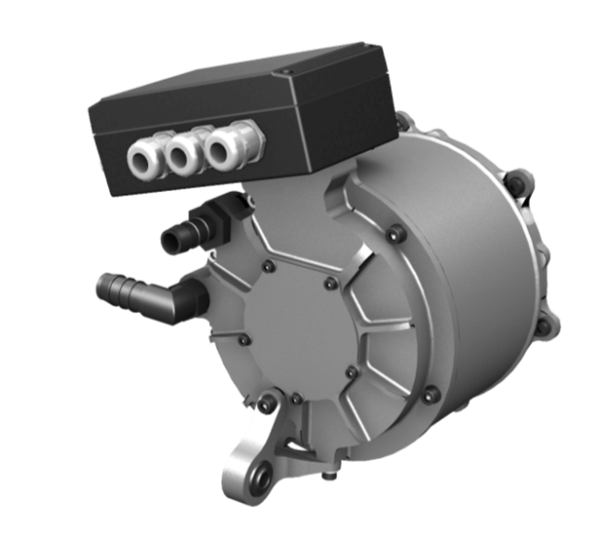
\includegraphics[width=0.4\paperwidth]{./Ressourcen/Praesentation/Bilder/Motor.png}
\end{textblock*}

\begin{textblock*}{0.6\paperwidth}[1,1](\textwidth + \PraesentationSeitenrand, \textheight - \PraesentationSeitenrand)%
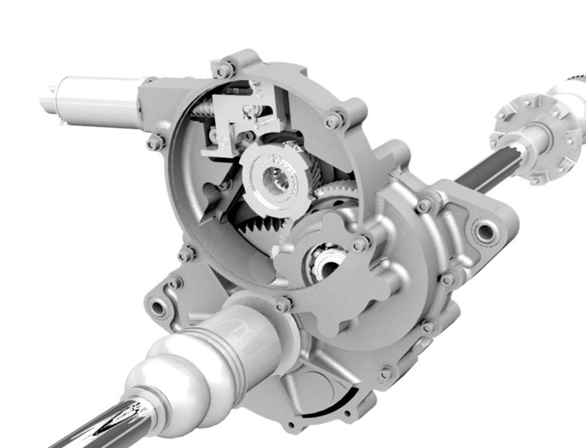
\includegraphics[width=0.6\paperwidth]{./Ressourcen/Praesentation/Bilder/Getriebe.png}
\end{textblock*}

\end{frame}
\clearpage


%%%%%%%%%%%%%%%%%%%%%%%%%%%%%%%%%%%
%% Folie: Bilder - formatfüllend %%
%%%%%%%%%%%%%%%%%%%%%%%%%%%%%%%%%%%
\begin{frame}
    \frametitle{Bilder Format füllend -- maximale Bildgröße}

\begin{minipage}[t][0cm]{\paperwidth}%
\hspace*{-\PraesentationSeitenrand}%

\includegraphics[width=\textwidth]{./Ressourcen/_Bilder/SternenhimmelQuer.jpg}
\end{minipage}
    
\end{frame}
\clearpage


%%%%%%%%%%%%%%%%%%%%%%%%%%%%%%%%%%%%%%%%%%%%%%%%%%%%%
%% Folie: Nicht Format füllende Bilder %%
%%%%%%%%%%%%%%%%%%%%%%%%%%%%%%%%%%%%%%%%%%%%%%%%%%%%%
\begin{frame}
    \frametitle{Nicht Format füllende Bilder}
    
Alternativ mit formatfüllendem Hintergrund: Weiß 5\% dunkler\newline
Beschriftungen können zusätzlich neben den Bildern angebracht werden

\begin{textblock*}{\paperwidth}[0,0](0cm, .4\textheight)%
Bilderklärung
\end{textblock*}

\begin{textblock*}{\paperwidth}[1,0](\textwidth, .4\textheight)%
\raggedleft%
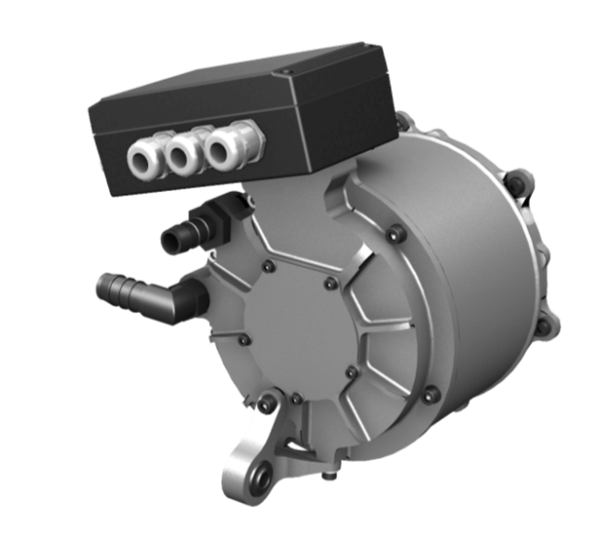
\includegraphics[height=0.5\textheight]{./Ressourcen/Praesentation/Bilder/Motor.png}
\end{textblock*}

\end{frame}
\clearpage


%%%%%%%%%%%%%%%%%%%%%%%%%%%%%%%%%%%%%%%%%%%%%%%%%%%%%
%% Folie: Tabelle - Ohne Rand 					   %%
%%%%%%%%%%%%%%%%%%%%%%%%%%%%%%%%%%%%%%%%%%%%%%%%%%%%%
\begin{frame}
    \frametitle{Tabelle -- Beispiel 1}
    
Tabelle ohne Farbe und kein Rand \\
innerer Seitenrand links 0 cm, um Faktor 1,75 skalierte Tabelle (für genug Zeilenabstand)

\raggedright
{
    \vspace*{0.3pt}
    \renewcommand{\arraystretch}{1.75} % skaliert die Tabelle auf die gewünschte Größe
    \begin{tabularx}{\textwidth}{@{} l @{\hspace{38.7mm}} X}
        Ø - Strecke & 39 km/Tag (14.360 km/Jahr) \\
        Ø - Geschwindigkeit & 25 km/h \\
        Ø - Verfügbare Ladezeit & 22 h/Tag \\
        Kosten   & Kleinwagen mit Verbrennungsmotor \\
        Einsatzgebiet   &  Stadt und Umland
    \end{tabularx}
}
\end{frame}


%%%%%%%%%%%%%%%%%%%%%%%%%%%%%%%%%%%%%%%%%%%%%%%%%%%%%
%% Folie: Tabelle - Mit Rand                       %%
%%%%%%%%%%%%%%%%%%%%%%%%%%%%%%%%%%%%%%%%%%%%%%%%%%%%%
\begin{frame}
    \frametitle{Tabelle -- Beispiel 2}
    
Tabelle ohne Farbe und mit Rand\\
automatische Zelleninnenabstände, um Faktor 1,75 skalierte Tabelle (für genug Zeilenabstand)

\raggedright
{
    \vspace*{0.3pt}
    \renewcommand{\arraystretch}{1.75} % skaliert die Tabelle auf die gewünschte Größe
    \begin{tabularx}{\textwidth}{| l @{\hspace{38.7mm}} | X |}
        \hline
        Ø - Strecke & 39 km/Tag (14.360 km/Jahr) \\ \hline
        Ø - Geschwindigkeit & 25 km/h \\ \hline
        Ø - Verfügbare Ladezeit & 22 h/Tag \\ \hline
        Kosten   & Kleinwagen mit Verbrennungsmotor \\ \hline
        Einsatzgebiet   &  Stadt und Umland \\ \hline
    \end{tabularx}
}
\end{frame}

\clearpage


%%%%%%%%%%%%%%%%%%%%%%%%%%%%%%%%%%%%%%%%%%%%%%%%%%%%%
%% Folie: Diagramme - Beispiel 1                   %%
%%%%%%%%%%%%%%%%%%%%%%%%%%%%%%%%%%%%%%%%%%%%%%%%%%%%%
\begin{frame}
    \frametitle{Diagramme -- Beispiel 1}

Nach Möglichkeit linksbündig bleiben \\
Unnötige Striche und Balken vermeiden

\begin{center}%
    \vspace*{-1cm}
    \begin{tikzpicture}
        \begin{axis}[
                % kein Abstand zwischen Balken:
                xbar=0,
                draw opacity=0,
                bar width=14,
                axis x line=none,
                axis line style={transparent},
                every tick/.style={transparent},
                xmin=0,
                width=\textwidth,
                height=.6\textheight,
                enlarge y limits=0.15,
                symbolic y coords={Kategorie 4,Kategorie 3,Kategorie 2,Kategorie 1},
                ytick=data,
                legend image code/.code={\draw[draw=none] (0cm,-0.12cm) rectangle (0.29cm,0.17cm);}, % Legenden-Symbol  
                legend columns=3,
                reverse legend,
                legend style={
                    fill=none,
                    draw=none,
                    /tikz/every odd column/.append style={column sep=0.07cm}, % Abstand zwischen Legenden-Symbol und Text
                    /tikz/every even column/.append style={column sep=0.8cm} % Abstand zwischen den Legendeneinträgen
                 },
                 legend to name=PraesentationDiagrammHorizontalLegende
            ]
            
            \addlegendentry{Datenreihe 3}
            \addlegendentry{Datenreihe 2}
            \addlegendentry{Datenreihe 1}
            
            \addplot[color=TUMBlauMittel, fill=TUMBlauMittel] coordinates {
                (1.2,Kategorie 1)
                (1.6,Kategorie 2)
                (2.2,Kategorie 3)
                (3.4,Kategorie 4)
            };
            
            \addplot[color=TUMBlauHell, fill=TUMBlauHell] coordinates {
                (1.5,Kategorie 1)
                (3.0,Kategorie 2)
                (1.0,Kategorie 3)
                (2.0,Kategorie 4)
            };
                
            \addplot[color=TUMBlauDunkel, fill=TUMBlauDunkel] coordinates {
                (3.0,Kategorie 1)
                (2.0,Kategorie 2)
                (2.5,Kategorie 3)
                (3.0,Kategorie 4)
            };
        \end{axis}
    \end{tikzpicture}
    \vspace*{-5mm}
    \ref*{PraesentationDiagrammHorizontalLegende}%
    
\end{center}
\end{frame}
\clearpage


%%%%%%%%%%%%%%%%%%%%%%%%%%%%%%%%%%%%%%%%%%%%%%%%%%%%%
%% Folie: Diagramme                                %%
%%%%%%%%%%%%%%%%%%%%%%%%%%%%%%%%%%%%%%%%%%%%%%%%%%%%%
\begin{frame}
    \frametitle{Diagramme}

\begin{center}
    \begin{tikzpicture}
        \begin{axis}[
                ybar=9.5,
                bar width=27.1,
                axis line style={transparent},
                every tick/.style={transparent},
                enlarge x limits=0.145, % X-Achse skalieren
                clip limits=true,
                ymin=0,
                ymax=6,
                width=\textwidth,
                height=.65\textheight,
                symbolic x coords={Kategorie 1,Kategorie 2,Kategorie 3,Kategorie 4},
                xticklabels={Kategorie 1,Kategorie 2,Kategorie 3,Kategorie 4},
                xtick=data,
                ytick={0,1,2,3,4,5,6},
                every tick label/.append style={font=\fontsize{13}{14}\selectfont},
                ymajorgrids,
                legend image code/.code={\draw[draw=none] (0cm,-0.12cm) rectangle (0.29cm,0.17cm);}, % Legenden-Symbol  
                legend columns=3,
                reverse legend,
                legend style={
                    font={\usebeamerfont{footnote}},
                    fill=none,
                    draw=none,
                    /tikz/every odd column/.append style={column sep=0.07cm}, % Abstand zwischen Legenden-Symbol
                    /tikz/every even column/.append style={column sep=0.8cm} % Abstand zwischen den Legendeneinträgen
                 },
                legend to name={PraesentationDiagrammVertikalLegende}
            ]
            
            \addlegendentry{Datenreihe 3}        
            \addlegendentry{Datenreihe 2}    
            \addlegendentry{Datenreihe 1}    
            
            \addplot[color=TUMBlauDunkel, fill=TUMBlauDunkel] coordinates {
                (Kategorie 1,4.2)
                (Kategorie 2,2.5)
                (Kategorie 3,3.5)
                (Kategorie 4,4.5)
            };
            
            \addplot[color=TUMBlauHell, fill=TUMBlauHell] coordinates {
                (Kategorie 1,2.3)
                (Kategorie 2,4.5)
                (Kategorie 3,1.8)
                (Kategorie 4,2.8)
            };
            
            \addplot[color=TUMBlauMittel, fill=TUMBlauMittel] coordinates {
                (Kategorie 1,2.0)
                (Kategorie 2,2.0)
                (Kategorie 3,3.0)
                (Kategorie 4,5.0)
            };        
        \end{axis}
     
    \end{tikzpicture}
    \vspace*{-5mm}
    \ref*{PraesentationDiagrammVertikalLegende}
   
\end{center}
\end{frame}
\clearpage

%%%%%%%%%%%%%%%%%%%%%%%%%%%%%%%%%%%%%%%%%%%%%%%%%%%%%


\begin{frame}
    \frametitle{Contents}
    \phantom{Spacing}
	\begin{PraesentationAufzaehlung}
		\item Introduction
		\item Component Modeling
		\begin{itemize}
			\item SMD Inductors
			\item SMD Capacitors
			\item SMD Resistors
		\end{itemize}
		\item Circuit Implementations
		\begin{itemize}
			\item Loop Circuit
			\item Patch Circuit
			\item Coplanar Circuit
			\item LC Bandpass Filters
			\item Lumped Wilkinson Divider
		\end{itemize}	
		\item Conclusion
	\end{PraesentationAufzaehlung}
\end{frame}

\begin{frame}
	\frametitle{Introduction}
	 Inverse source solvers are computational methods used for solving inverse scattering problems \cite{381063}.
	 
	 In the context of electromagnetics the solver computes equivalent current distributions that produce the observed fields from a set of measurement samples \cite{4812237}.
	 
	 The solver can then perform important computations such as near-field to near-field or far-field transformations \cite{4812237}.
	 
	 Some numerical techniques for solving inverse scattering problems based on integral equations suffer from a low frequency breakdown \cite{8293221}.
	 
	 \textcolor{TUMBlau}{The goal of this work is to design test circuits with diverse near-field patterns for evaluating the low frequency breakdown of an inverse source solver.}
\end{frame}

\begin{frame}
	\PraesentationUeberschriftZweizeilig{Component Modeling}{SMD Inductors} 
	\textbf{Equivalent Circuit}\\
	\begin{columns}
		\column{0.5\textwidth}
		\begin{figure}
			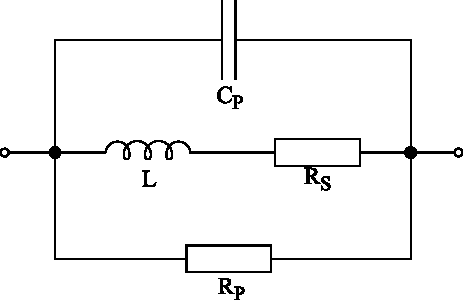
\includegraphics[width=0.75\textwidth, center]{inductor_eqv.pdf}
		\end{figure}
		\column{0.5\textwidth}
		\vspace{5em}
		\captionof{figure}{Equivalent circuit diagram of inductors in Spice simulators.}
	\end{columns}
	\vspace{-15pt}
	In the above circuit $R_\mathrm{S}$ models the DC resistance of the coil, $R_\mathrm{P}$ models losses due to a magnetic core, and $C_\mathrm{P}$ models the capacitive coupling between the windings, as well as the coupling between the windings and both the shield and the core.
	
	Self resonance frequency of the inductor:
	\begin{equation}
		f_{\mathrm{SR}} = \frac{1}{2\pi\sqrt{LC_\mathrm{P}}}
	\end{equation}
\end{frame}

\begin{frame}
	\frametitle{SMD Inductors - Air Core Inductors} 
	\textbf{Modeling of 744912210 Aircore Inductor by Würth Elektronik}\\
	\begin{columns}
		\column{0.4\textwidth}
		\begin{figure}
			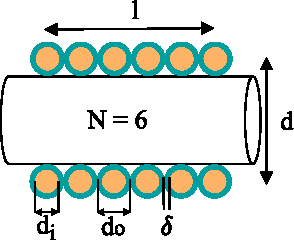
\includegraphics[width=0.75\textwidth, right]{singlelayer.pdf}
		\end{figure}
		\column{0.6\textwidth}
		\vspace{5.25em}
		\captionof{figure}{Geometry parameters of a single layer air core inductor.}
	\end{columns}
	\vspace{-15pt}
	The geometry parameters are predicted using the inductance formula for single layer short coils:
	\begin{equation}\label{eqn:aircoil1}
		L_\mathrm{s} = N^2\mu_0\frac{\pi (d/2)^2}{l}k \,,
	\end{equation}
	whereas $k$ is the Nagaoka correction factor \cite{nagaoka} and calculated with
	\begin{equation}
		k = \frac{4}{3\pi}\frac{1}{\kappa'}\left(\frac{\kappa'^2}{\kappa^2}(K(\kappa)-E(\kappa))+E(\kappa)-\kappa\right)\,,
		\quad \mathrm{with} \quad
		\kappa = \frac{d}{d^2+l^2}
		\quad \mathrm{and} \quad
		\kappa' = \frac{l}{d^2+l^2}\,.
	\end{equation}
	Here $K(\cdot)$ and $E(\cdot)$ are the complete elliptical integrals of the first and second kind, respectively.
\end{frame}

\begin{frame}
	\frametitle{SMD Inductors - Air Core Inductors} 
	Applying Rosa's round wire correction, the total inductance becomes:
	\begin{equation}
		L = L_\mathrm{s} - \mu_0\frac{d}{2}N(k_\mathrm{s}+k_\mathrm{m})\,,
	\end{equation}
	where $k_m$ and $k_s$ are tabularized in \cite{rosa}. The DC resistance of the inductor is calculated using
	\begin{equation}  \label{eqn:aircoilson1}
		R_\mathrm{S} = \rho\frac{l_\mathrm{w}}{\pi (d/2)^2}\,,
		\quad \text{with wire length} \quad 
		l_\mathrm{w} = N\sqrt{(\pi d)^2+(l/N)^2}\,,
	\end{equation}
	and the parasitic resistance of the inductor is calculated using Medhurst's empirical equation in \cite{medhurst}: 
	\begin{equation} \label{eqn:aircoilson2}
		C_\mathrm{P} = \frac{4\varepsilon_0l}{\pi}\left(1+0.71\frac{d}{l}+2.4\left(\frac{d}{l}\right)\strut^{1.5}\right)\,.
	\end{equation}
	The feasibility of the predicted geometry is checked using \eqref{eqn:aircoilson1}, \eqref{eqn:aircoilson2} by comparing the results to the manufacturer's data. Subsequently a valid coil geometry is decided.
	\begin{columns}
		\column{0.4\textwidth}
		\centering
		\begin{figure}
			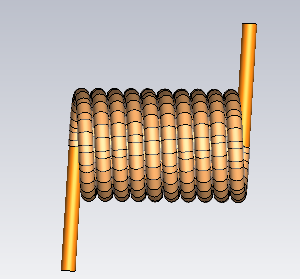
\includegraphics[width=0.45\textwidth, right]{744912210.png}
		\end{figure}
		\column{0.5\textwidth}
		\vspace{4em}
		\captionof{figure}{3D model of the air core inductor 744912210 in CST.}
	\end{columns}
\end{frame}

\begin{frame}
	\frametitle{SMD Inductors - Air Core Inductors}
	\phantom{text}
	\begin{table}[ptbh]
		\centering
		\begin{tabular}{|c c c c c|}
			\hline
			 $N$ & $d$ (\SI{}{\milli\meter}) & $l$ (\SI{}{\milli\meter}) & $d_\mathrm{i}$ (\SI{}{\milli\meter}) & $\delta$ (\SI{}{\milli\meter})\\
			\hline
			10 & 2.6 & 4.5 & 0.4 & 0.0185\\
			\hline
		\end{tabular} 
		\caption{Valid geometry from the analytical equations for the air core inductor 744921210.}
		\label{tab:valid_geom}
	\end{table}
	\begin{table}[ptbh]
		\centering
		\begin{tabular}{|c|c| c c c c|}
			\hline
			Model number& Results from & $L\,(\SI{}{\nano\henry})$ & $R_\mathrm{S}\,(\SI{}{\milli\ohm})$ & $C_\mathrm{P}\,(\SI{}{\pico\farad})$ & $f_\mathrm{SR}\,(\SI{}{\giga\hertz})$\\
			\hline
			&Equations & 105 & 12.1 & 0.125& 1.390\\
			744912210 & CST & 100 & 12.8 &  0.131 & 1.389\\
			&Datasheet & $100\pm5\%$ & $< 12.3$ & $< 0.176$ & $> 1.2$\\
			\hline
		\end{tabular} 
		\caption{Important values obtained from analytical equations and from CST are compared with the data provided by the manufacturer for the air core inductor 744912210.}
		\label{tab:air_core_results}
	\end{table}
\end{frame}

\begin{frame}
	\frametitle{SMD Inductors - Important Ferrite Core Concepts}
	\textbf{Effective relative permeability}\\
	For open cores the ratio between the inductance with and without a ferrite core ($L_\mathrm{f}/L_\mathrm{air} =: \mu_\mathrm{r,eff}$) can be much lower than the relative permeability $\mu_\mathrm{r}$ of the core, depending on the core geometry. In \cite{snelling} following formula is introduced for calculating $\mu_\mathrm{r,eff}$:
	\begin{equation} \label{eqn:demag}
		\mu_{\mathrm{r,eff}} = \frac{\mu_\mathrm{r}}{1+D(\mu_\mathrm{r}-1)}\,,
	\end{equation}
	where D is the demagnetization factor. For cylindrical rods it is given in the graphs below.
	\vspace{-15pt}
	\begin{figure}
		\centering
		\begin{tabular}{cc}
			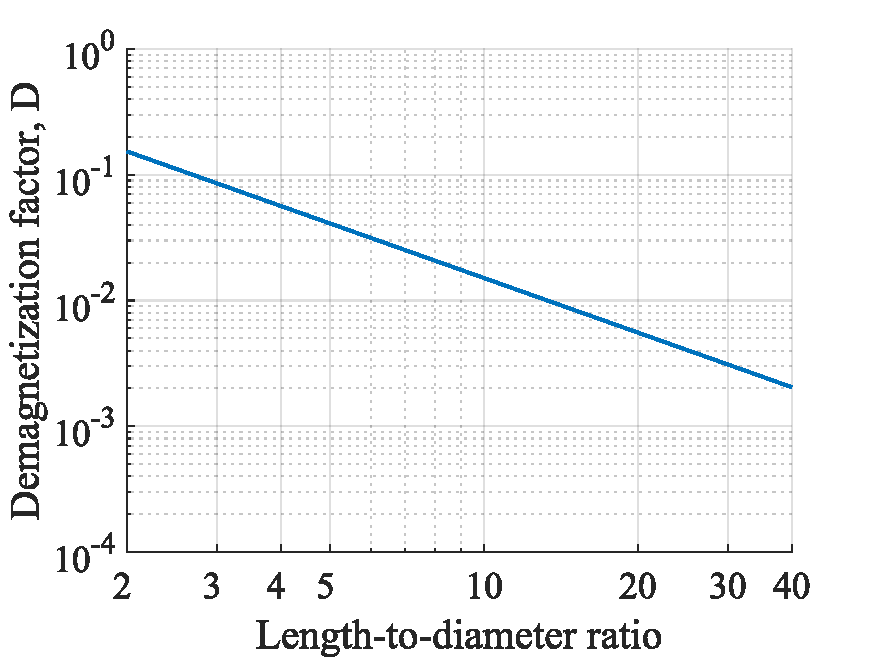
\includegraphics[width=0.33\textwidth]{demag.pdf}&
			\hspace{25pt}
			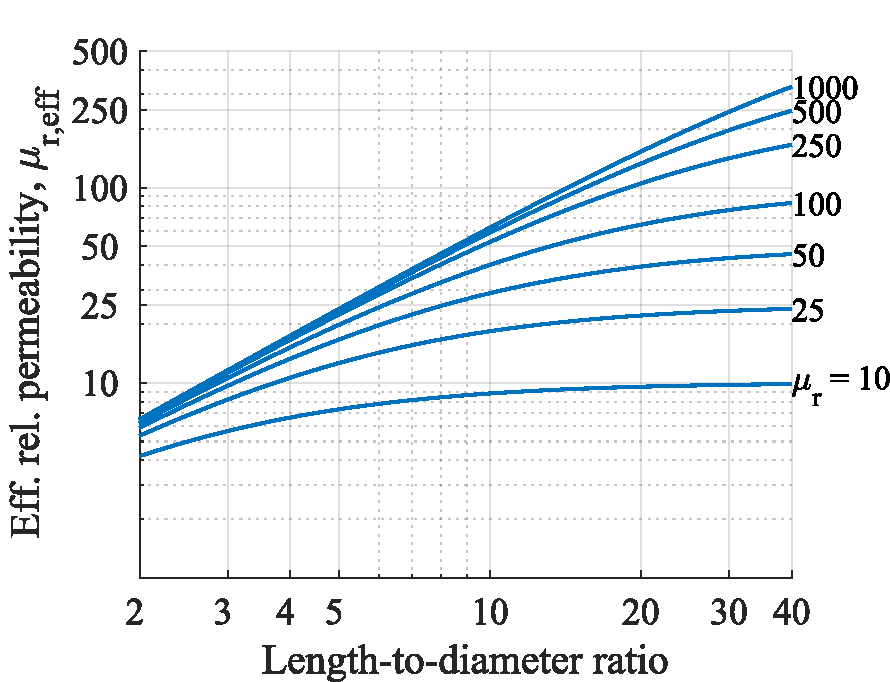
\includegraphics[width=0.33\textwidth]{murod.pdf}
		\end{tabular}
		\caption{Demagnetization factor of a cylindrical core depending on the length-to-diameter ratio (left). Eff. rel. permeability $\mu_\mathrm{r,eff}$ of a cylindrical magnetic core depending on the relative permeability and the length-to-diameter ratio (right).}
	\end{figure}
\end{frame}

\begin{frame}
	\frametitle{SMD Inductors - Important Ferrite Core Aspects}
	\textbf{Core saturation}\\
	In the equation
	\begin{equation}\label{eqn:magnetization}
		\vec{B} = \mu_0\vec{H}+\mu_0\vec{M}
	\end{equation}
	the contribution of $\mu_0\vec{M}$ stops increasing for very large $\vec{H}$ and $\mu_\mathrm{r}$ drops to 1. 
	\vspace{-15pt}
	\begin{figure}
		\centering
		\begin{tabular}{cc}
			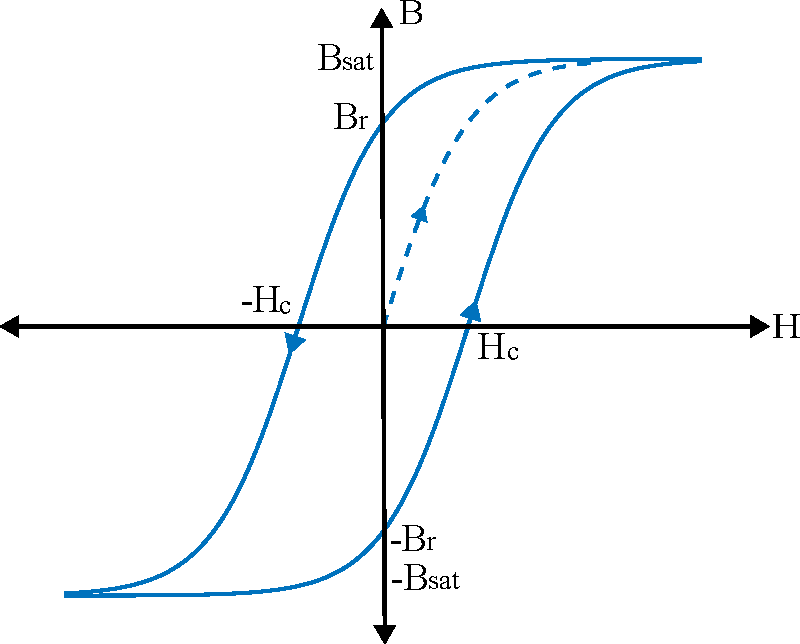
\includegraphics[width=0.33\textwidth]{mag_curve.pdf}&
			\hspace{25pt}
			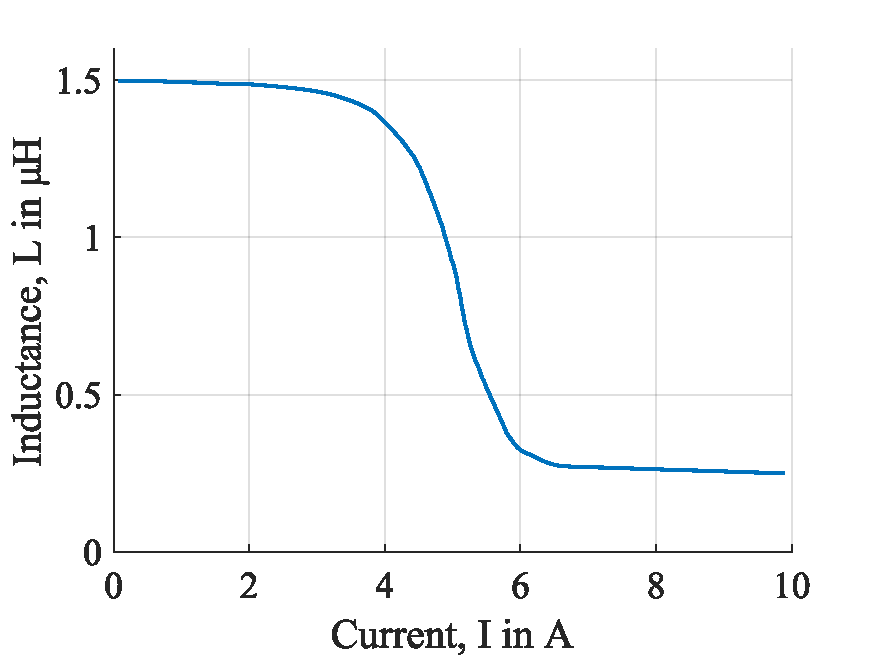
\includegraphics[width=0.33\textwidth]{0450015_ind.pdf}
		\end{tabular}
		\caption{Qualitative magnetization curve for an arbitrary magnetic core (left). Inductance of 7440450015 drum core inductor from Würth Elektronik depending on the current (right).}
	\end{figure}
\end{frame}

\begin{frame}
	\frametitle{SMD Inductors - Important Ferrite Core Aspects}
	\textbf{Dispersion of relative permeability}
	\begin{equation} \label{eqn:disp1}
		\underline{\mu_\mathrm{r}}(\omega) = 1 + \underline{\chi_\mathrm{sp}}(\omega)  +  \underline{\chi_\mathrm{dw}}(\omega)\,,
	\end{equation}
	\begin{equation} \label{eqn:disp2}
		\underline{\mu_\mathrm{r}}(\omega) = 1 + \frac{(\omega_\mathrm{sp}+j\omega\alpha)\omega_\mathrm{sp}\chi_\mathrm{sp}^0}{(\omega_\mathrm{sp}+j\omega\alpha)^2-\omega^2} +  \frac{\omega_\mathrm{dw}^2\chi_\mathrm{dw}^0}{\omega_\mathrm{dw}^2-\omega^2+j\omega\beta}\,,
		\quad \text{for } \alpha \gg 1,\, \underline{\chi_\mathrm{sp}}\text{ becomes} \quad
		\frac{\chi_\mathrm{sp}^0}{1+j\omega\tau}\,,
	\end{equation}
	where $\chi_\mathrm{sp}^0$, $\chi_\mathrm{dw}^0$ are low frequency susceptibilities of spin rotation and domain wall motion, $\omega_\mathrm{sp}$, $\omega_\mathrm{dw}$ are the corresponding resonance frequencies, $\alpha$, $\beta$ are damping factors and $\tau$ is the relaxation time constant \cite{landau, tsutaoka, aee423}.
	\vspace{-15pt}
	\begin{columns}
		\column{0.35\textwidth}
		\begin{figure}
			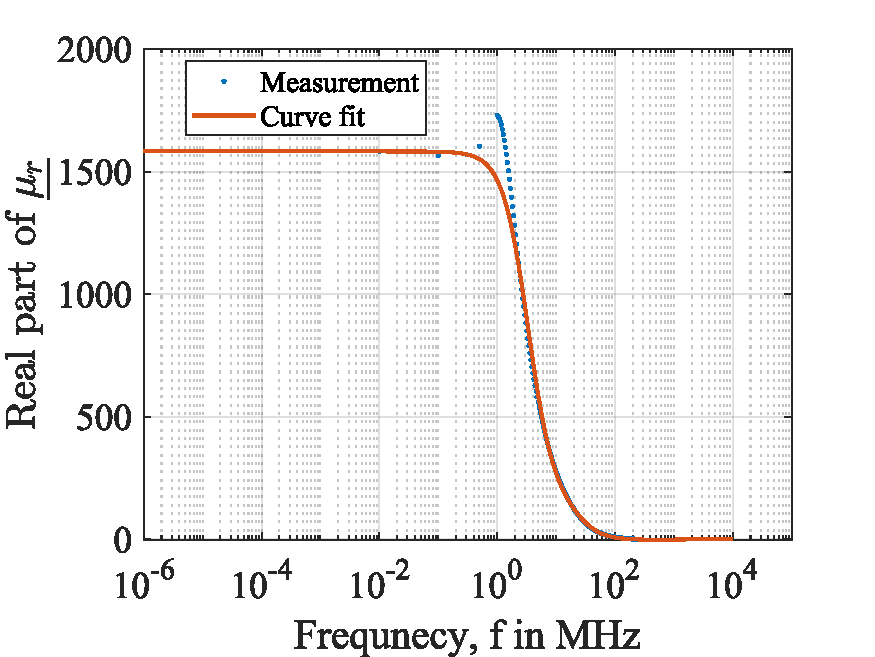
\includegraphics[width=\textwidth]{fit1.pdf}
		\end{figure}
		\column{0.35\textwidth}
		\begin{figure}
			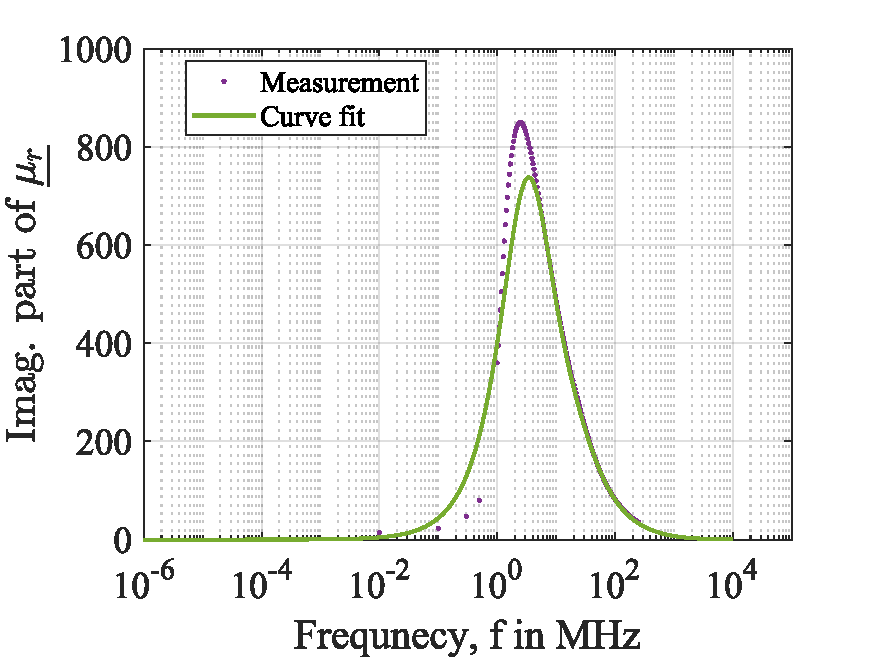
\includegraphics[width=\textwidth]{fit2.pdf}
		\end{figure}
		\column{0.3\textwidth}
		\vspace{1.25em}
		\captionof{figure}{Complex permeability of the Fair-Rite 15~Material is fitted with \eqref{eqn:disp2}. The following parameters are obtained from the particle swarm optimizer in MATLAB: $\chi_\mathrm{sp}^0 = 1433$, $\omega_\mathrm{sp} = \SI[per-mode=symbol]{9e9}{\radian\per\second}$, $\alpha = 427.7 $; $\chi_\mathrm{dw}^0 = 147$, $\omega_\mathrm{dw} = \SI[per-mode=symbol]{1.1e9}{\radian\per\second}$, $\beta = \SI[per-mode=symbol]{8.3e9}{\radian\per\second}$}
	\end{columns}
\end{frame}

\begin{frame}
	\frametitle{SMD Inductors - Drum Core Inductors}
	\textbf{Modeling of 7440450015 and 744045002 drum core inductors from Würth Elektronik.}\\
	\begin{figure}
		\centering
		\begin{tabular}{cc}
			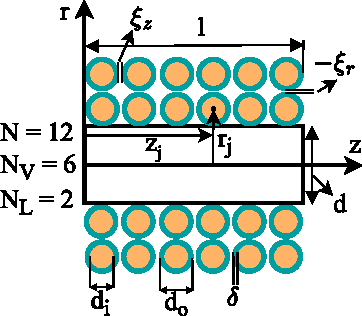
\includegraphics[width=0.31\textwidth]{multilayer.pdf}
			\hspace{25pt}
			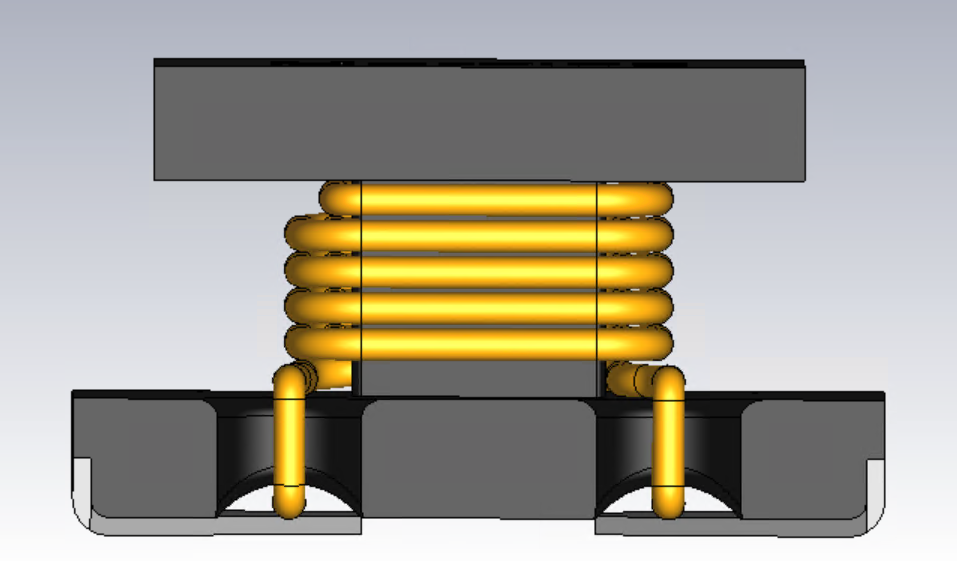
\includegraphics[width=0.33\textwidth]{744045001.png}&
		\end{tabular}
		\caption{Geometry parameters of multilayer inductors (left). 3D CAD model of 744045001 from Würth Elektronik (right).}
	\end{figure}
	\vspace{-25pt}
	In the first step, the core is ignored. The multilayer coil is modeled similar to \cite{6732932}. The geometry parameters of the coil is predicted using
	\begin{equation}
		L_\mathrm{air} = \sum_{j=0}^{N}L_j + \sum_{j=0}^{N}\sum_{\substack{k=0 \\ k\neq j}}^{N}M_{jk}\,,
	\end{equation}
	whereas $L_j$ is the self-inductance of the $j$-th winding and $M_{jk}$ is the mutual inductance between the $j$-th and $k$-th windings and $L_\mathrm{air}$ is taken from the inductance vs.current graphs in datasheets~\cite{6732932}.
\end{frame}

\begin{frame}
	\frametitle{SMD Inductors - Drum Core Inductors}
	From Grover's book~\cite{grover2013}, for a square winding with side length $r_j$ and wire radius $d_i/2$, the self inductance is
	\begin{equation}  \label{eqn:multilayer_eqn2}
		L_j = \mu_0\frac{2r_j}{\pi}\left(\ln\left(\frac{2r_j}{(d_i/2)}\right) - 0.77401\right)\,.
	\end{equation}
	and from Cheng and Shu's paper~\cite{cheng}, for two coaxial square current filaments with side lengths $2a$ and $2c$ and distance apart $z$, the mutual inductance is
	\begin{equation}
		\begin{aligned}
		    M = \frac{2\mu_0}{\pi}\Bigg[&
		    \sqrt{2(a+c)^2+z^2}+\sqrt{2(a-c)^2+z^2}-2\sqrt{2a^2+2c^2+z^2} \\ &-(a+c)\arctanh{\left(\frac{a+c}{\sqrt{2(a+c)^2+z^2}}\right)}-(a-c)\arctanh{\left(\frac{a-c}{\sqrt{2(a-c)^2+z^2}}\right)} \\
		    &+(a+c)\arctanh{\left(\frac{a+c}{\sqrt{2a^2+2c^2+z^2}}\right)}+(a-c)\arctanh{\left(\frac{a-c}{2a^2+2c^2+z^2}\right)}\Bigg]\,.
		\end{aligned}
	\end{equation}
	To make this equation compatible with the model used in this work and thus to obtain $M_{jk}$, $a$ needs to be replaced with $r_j$, $c$ needs to be replaced with $r_k$, and $z$ needs to be replaced with $\abs{z_j - z_k}$.
\end{frame}
	
\begin{frame}
	\frametitle{SMD Inductors - Drum Core Inductors}
	The DC resistance of a multilayer coil can be calculated with
	\begin{equation} \label{eqn:multilayer_eqn4}
		R_\mathrm{S} = \rho_\mathrm{c}\frac{l_\mathrm{w}}{\pi(d_\mathrm{i}/2)^2}\,, 
		\quad \text{with} \quad
		l_\mathrm{w} = \sum_{j=0}^{N}\left(4\sqrt{(2r_j)^2+(p/4)^2}\right)\,,
	\end{equation}
	where $p = d_\mathrm{o}+\xi_z$ is the pitch of the windings.
	
	Finally the inductors are implemented in CST. The relative permeabilities are determined with a parameter sweep. The dispersion had to be modeled with the 1st order Debye model and the parameter $\tau$ is optimized such that the parallel resistances $R_\mathrm{P}$ match together.
	\vspace{-15pt}
	\begin{table}[ptbh]
		\centering
		\begin{tabular}{|c|c c c c c c c c c|}
			\hline
			Inductor & $L_\mathrm{f}\,(\SI{}{\micro\henry})$ & $L_{\mathrm{air}}\,(\SI{}{\micro\henry})$ & $\mu_\mathrm{r}$ & $\mu_\mathrm{r,eff}$ & D & $\tau\,(\SI{}{\nano\second})$ & $N$ & $N_\mathrm{L}$ & $N_\mathrm{V}$\\
			\hline
			7440450015 & 1.50 & 0.216 & 22 & 6.94 & 0.11 & 0.95  & 12 & 2 & 6\\
			744045002 & 2.23 & 0.333 & 25 & 6.67 & 0.11 & 0.65  & 15 & 3 & 5\\
			\hline
		\end{tabular}
		\begin{tabular}{|c| c c c c c c c|}
			\hline
			Inductor & $l\,(\SI{}{\milli\meter})$ & $d\,(\SI{}{\milli\meter})$ & $d_\mathrm{i}\,(\SI{}{\milli\meter})$ & $\delta\,(\SI{}{\milli\meter})$ & $d_\mathrm{o}\,(\SI{}{\milli\meter})$ & $\xi_z\,(\SI{}{\milli\meter})$ & $\xi_r\,(\SI{}{\milli\meter})$\\
			\hline
			7440450015 & 1.08 & 1.4 & 0.16 & 0.01 & 0.18 & 0.005 & -0.005 \\
			744045002 & 1.00 & 1.4 & 0.18 & 0.01 & 0.20 & 0.005  & -0.005 \\
			\hline
		\end{tabular}
		\caption{Geometry parameters as well as material parameters predicted for 7440450015 and 744045002.}
		\label{tab:drum_core_result}
	\end{table}
\end{frame}

\begin{frame}
	\frametitle{SMD Inductors - Drum Core Inductors}
	\begin{figure}
		\centering
		\begin{tabular}{cc}
			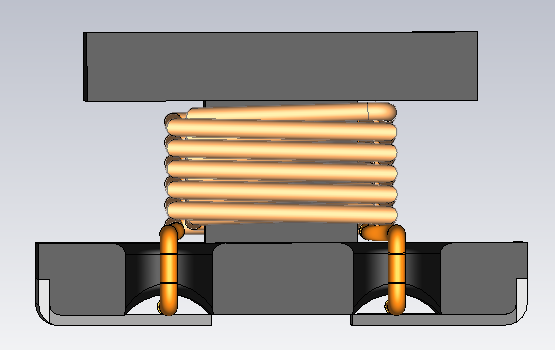
\includegraphics[width=0.3\textwidth]{7440450015.png}
			\hspace{25pt}
			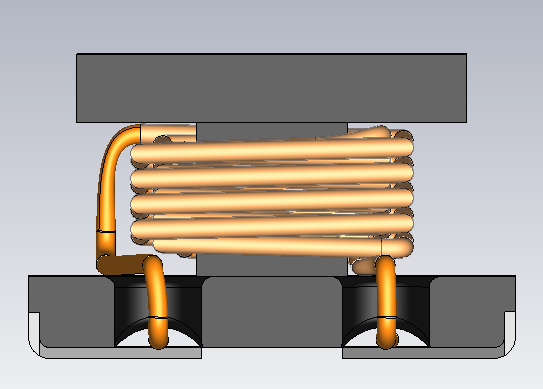
\includegraphics[width=0.2625\textwidth]{744045002.png}
		\end{tabular}
		\caption{3D models of the inductors in CST. 7440450015 on the left and 744045002 on the right.}
	\end{figure}
	\vspace{-15pt}
	\begin{table}[ptbh]
		\centering
		\begin{tabular}{|c|c|c c c c c c|}
			\hline
			Model number & Results from & $L_\mathrm{f}\,(\SI{}{\micro\henry})$ & $L_\mathrm{air}\,(\SI{}{\micro\henry})$ & $R_\mathrm{S}\,(\SI{}{\ohm})$ & $R_\mathrm{P}\,(\SI{}{\ohm})$ & $C_\mathrm{P}\,(\SI{}{\pico\farad})$ & $f_\mathrm{SR}\,(\SI{}{\mega\hertz})$\\
			\hline
			& Equations & -- & 0.229 & 0.073 & -- & -- & --\\
			\multirow{ 2}{*}{7440450015} & CST & 1.5 & 0.216 & 0.077 & 3330.8 & 0.834 & 145\\
			& LTSpice & 1.5 & -- & 0.072 & 3303.9 & 1.155 & 121\\
			& Datasheet & $1.5\pm20\%$ & 0.235 & < 0.090 & -- & $\approx 1$ & $\approx 130$\\
			\hline
			& Equations & -- & 0.404  & 0.082 & -- & -- & --\\
			\multirow{ 2}{*}{744045002} & CST & 2.23 & 0.333 & 0.086 & 8002.9 & 0.72 & 123\\
			& LTSpice & 2.2 & --  & 0.088 & 7826.2 & 0.863 & 120\\
			& Datasheet & $2.2\pm20\%$ & 0.32 & < 0.110 & -- & $\approx1.8$ & $\approx80$\\
			\hline
		\end{tabular} 
		\caption{Important results from analytical equations and from CST simulations are compared with the data provided by the manufacturer, taken from the datasheets and the Spice models.}
		\label{tab:calc_compare}
	\end{table}
\end{frame}
	
\begin{frame}
	\frametitle{SMD Inductors - Drum Core Inductors}
	\begin{figure}
		\begin{tabular}{cc}
			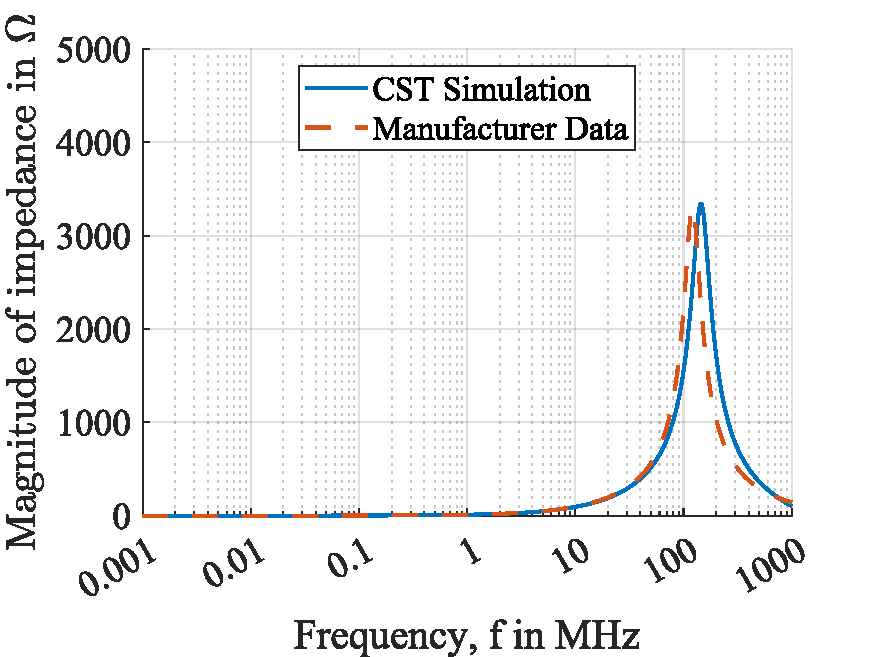
\includegraphics[width=0.4\textwidth]{cstvsmanuf_0015.pdf}
			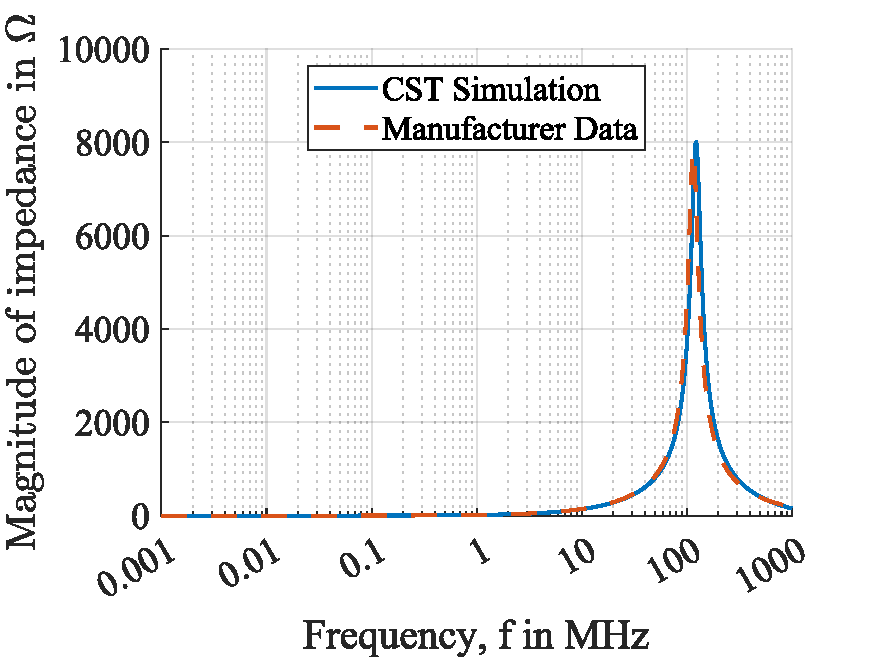
\includegraphics[width=0.4\textwidth]{cstvsmanuf_002.pdf}
		\end{tabular}
		\caption{Comparison between the $\abs{\underline{Z_\mathrm{L}}(\omega)}$ values from CST and simulation of manufacturer's Spice model for 7440450015 (left) and for 744045002 (right).}
	\end{figure}
\end{frame}

\begin{frame}
	\frametitle{SMD Capacitors} \textbf{Inner structure and equivalent circuit}
	\begin{figure}
		\centering
		\begin{tabular}{cc}
			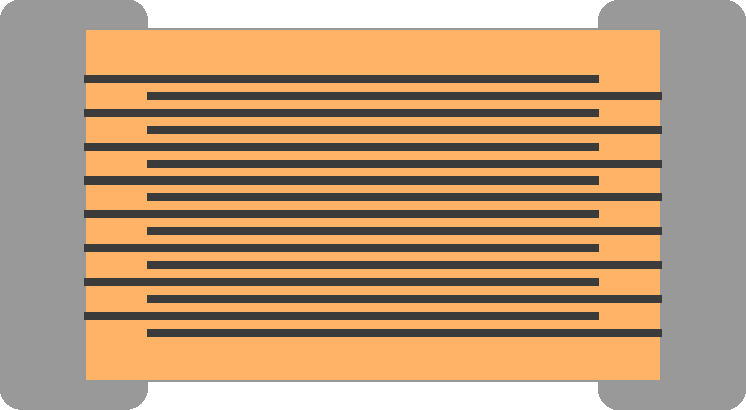
\includegraphics[width=0.3\textwidth]{mlcc.pdf}
			\hspace{25pt}
			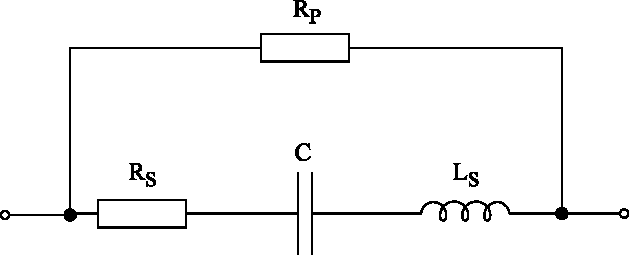
\includegraphics[width=0.4\textwidth]{capacitor_eqv.pdf}
		\end{tabular}
		\caption{Inner structure of a multi-layer ceramic capacitor (MLCC) (left) and its equivalent circuit in Spice simulators (right).}
	\end{figure}
	\vspace{-15pt}
	An MLCC consists of stacked metal layers in a ceramic dielectric. Adjacent metal layers are connected to opposite electrodes, forming a parallel connection so that total capacitance becomes $N_{\mathrm{C}}\varepsilon_0\varepsilon_\mathrm{r}A/d$, where $N_{\mathrm{C}}$ is the number of layers \cite{5482787}.

	In the equivalent circuit above $R_\mathrm{S}$ models the losses in the dielectric, $R_\mathrm{P}$ models the current leakage through the dielectric and $L_\mathrm{S}$ models the inductance of metal connections.
\end{frame}

\begin{frame}
	\frametitle{SMD Capacitors} \textbf{3D modeling}
	\begin{figure}
		\centering
		\begin{tabular}{cc}
			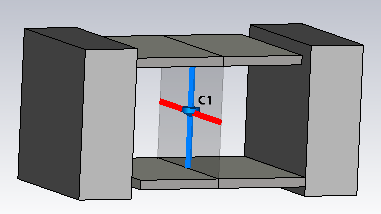
\includegraphics[width=0.3\textwidth]{885342008003.png}
			\hspace{25pt}
			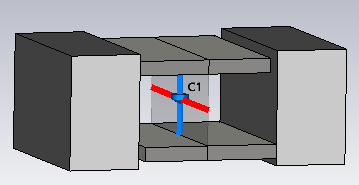
\includegraphics[width=0.3\textwidth]{885012007087.png}
		\end{tabular}
		\caption{Two examples out of various capacitor models implemented in CST. 885342008003 (left) and 885012007087 (right).}
	\end{figure}
	\vspace{0pt}
	For the 3D modeling of MLCCs the brick modeling approach is followed in accordance with Modelithics and \cite{8094717}.
	
	The external geometry of the component is exact. The internal part of the component contains a lumped element that includes the manufacturer-released Spice model.
\end{frame}

\begin{frame}
	\frametitle{SMD Resistors} \textbf{Inner structure, equivalent circuits and 3D modeling}\\
	\begin{figure}
		\centering
		\begin{tabular}{ccc}
			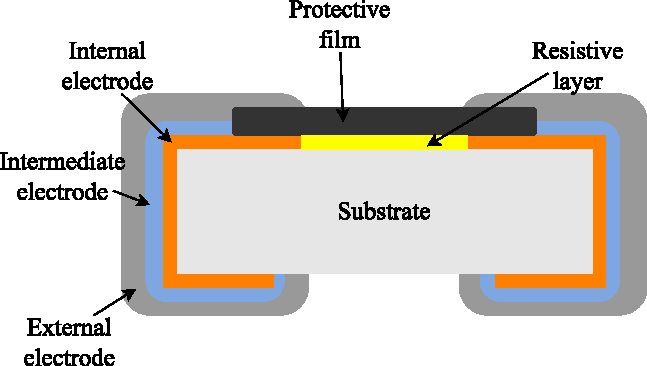
\includegraphics[width=0.3\textwidth]{resistor.pdf}
			\hspace{25pt}
			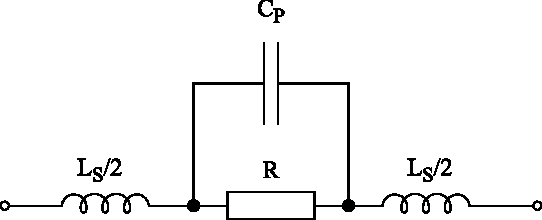
\includegraphics[width=0.3\textwidth]{resistor_eqv1.pdf}
			\hspace{25pt}
			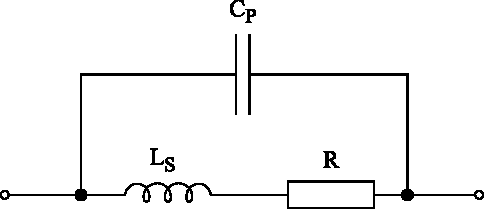
\includegraphics[width=0.3\textwidth]{resistor_eqv2.pdf}
		\end{tabular}
		\caption{Inner structure of a thin-/thick-film resistor (left), its equivalent circuit for $R \lessapprox \SI{100}{\ohm}$ (middle) and for  $R \gtrapprox \SI{100}{\ohm}$ (right) \cite{hft}}
	\end{figure}
	\vspace{-25pt}
	The impedance of the resistor in the middle continuously increases with increasing frequency, whereas the impedance of the resistor on the left contentiously decreases.
	\vspace{-20pt}
	\begin{columns}
		\column{0.3\textwidth}
		\begin{figure}
			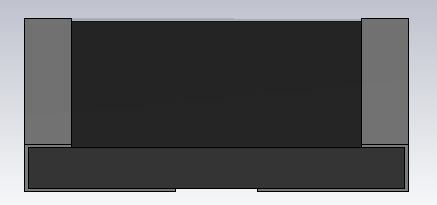
\includegraphics[width=\textwidth]{RCP1206W50R0GEB.png}
		\end{figure}
		\column{0.3\textwidth}
		\begin{figure}
			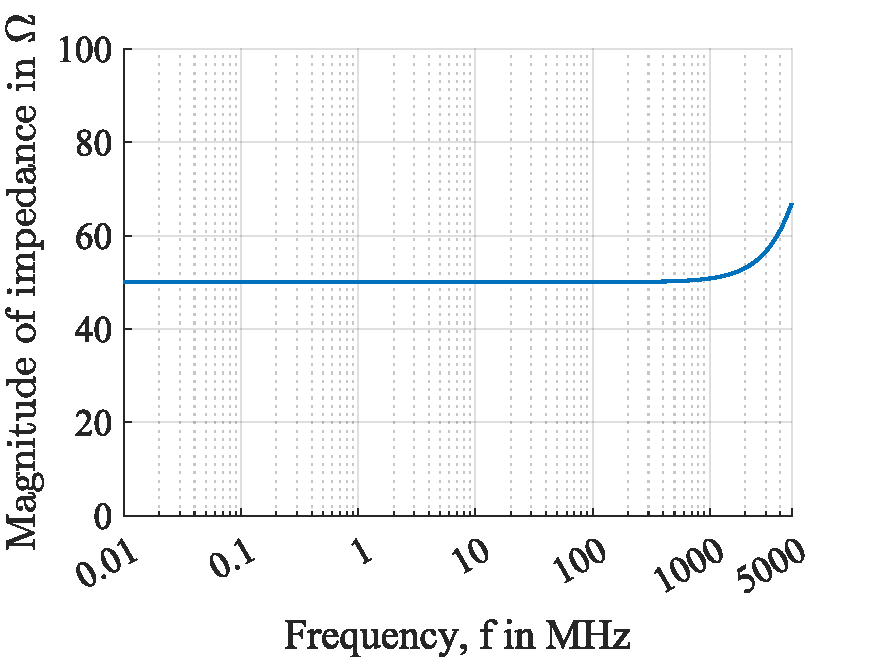
\includegraphics[width=\textwidth]{rcp.pdf}
		\end{figure}
		\column{0.3\textwidth}
		\vspace{3em}
		\captionof{figure}{The \SI{50}{\ohm} resistor RCP1206W50R0GEB modeled in CST (left) and its impedance depending on the frequency (right).}
	\end{columns}
\end{frame}

\begin{frame}
	\PraesentationUeberschriftZweizeilig{Circuit Implementations}{Loop Circuit}
	\begin{figure}
		\centering
		\begin{tabular}{ccc}
			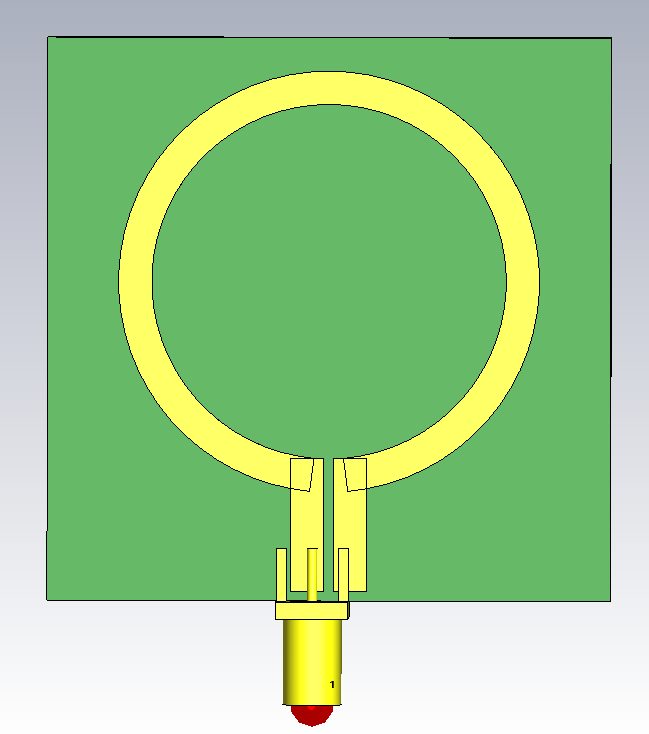
\includegraphics[width=0.19\textwidth]{loop.png}&
			\hspace{25pt}
			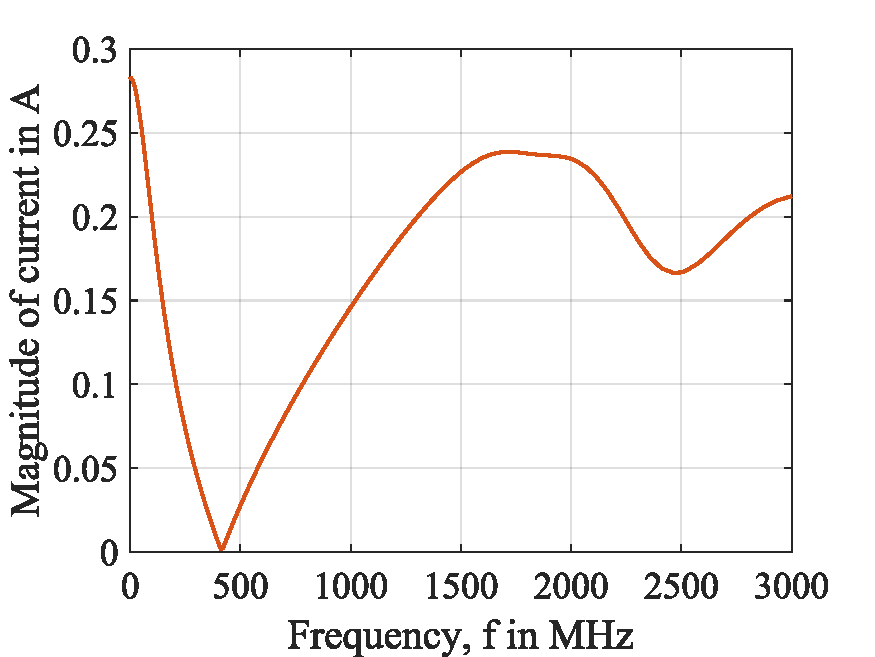
\includegraphics[width=0.3\textwidth]{loop_cur.pdf}&
			\hspace{25pt}
			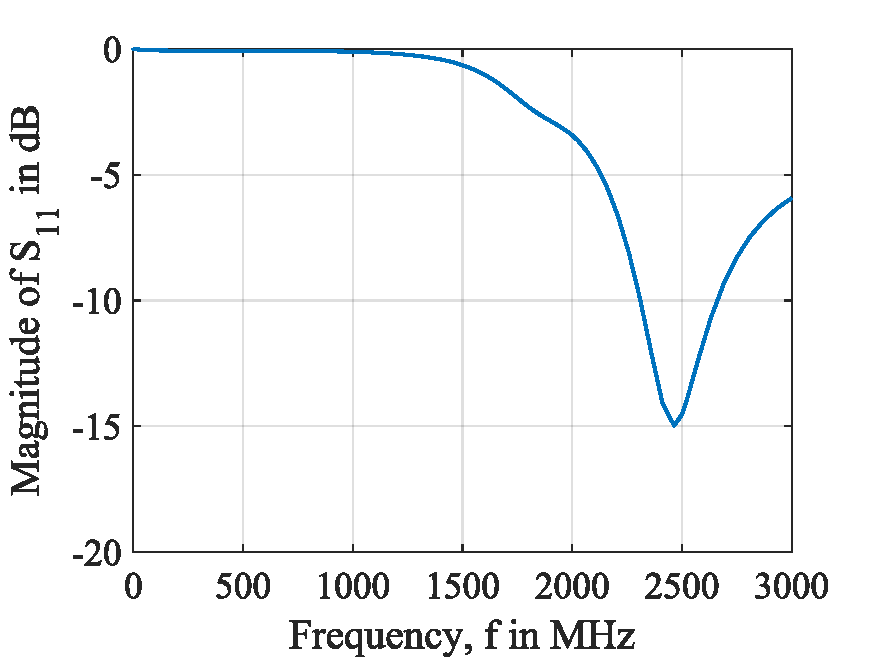
\includegraphics[width=0.3\textwidth]{loop_s11.pdf}
		\end{tabular}
		\caption{Loop circuit implemented in CST (left), the magnitude of current through it (middle) and magnitude of the $S_{11}$-parameter (right).}
	\end{figure}
	The circuit is implemented on a $\SI{50.8}{\milli\meter} \times \SI{50.8}{\milli\meter}$ Rogers RO4003C PCB without a ground plane at the bottom. The inner radius of the loop is \SI{17.5}{\milli\meter} and the wire width is \SI{3}{\milli\meter}.
\end{frame}

\begin{frame}
	\frametitle{Loop Circuit}
	\begin{columns}
		\column{0.6\textwidth}
		\begin{figure}
			\centering
			\begin{tabular}{c}
				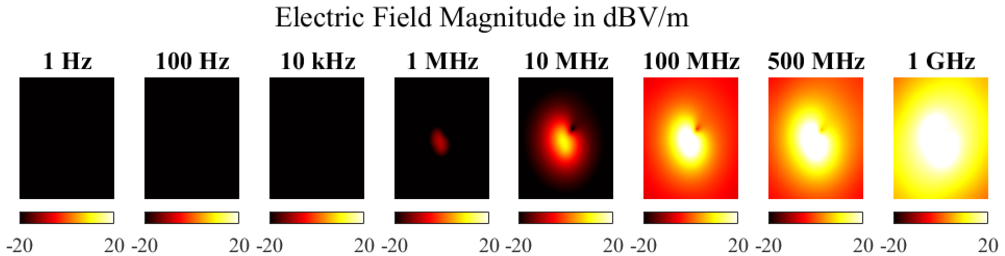
\includegraphics[width=\textwidth]{loop1.pdf}\\
				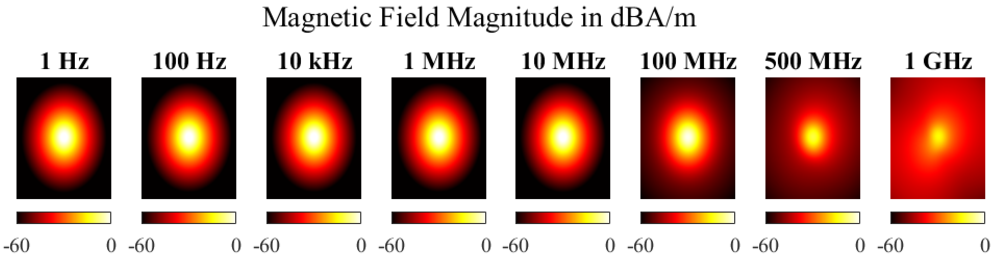
\includegraphics[width=\textwidth]{loop2.pdf}
			\end{tabular}
		\end{figure}
		\column{0.4\textwidth}
		\vspace{8em}
		\captionof{figure}{Near-field simulation results collected \SI{3}{\centi\meter} above the circuit in a $\SI{40}{\centi\meter} \times \SI{40}{\centi\meter}$ plane for the loop circuit.}
	\end{columns}
	\vspace{-20pt}
	\begin{columns}
		\column{0.8\textwidth}
		\begin{figure}
			\begin{tabular}{ccc}
				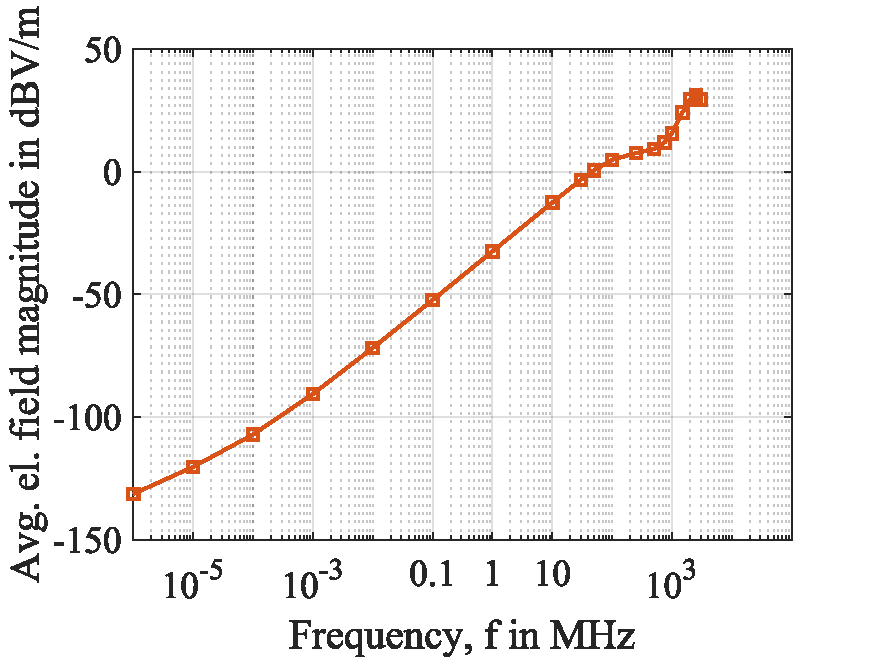
\includegraphics[width=0.32\textwidth]{loop_ave.pdf}&
				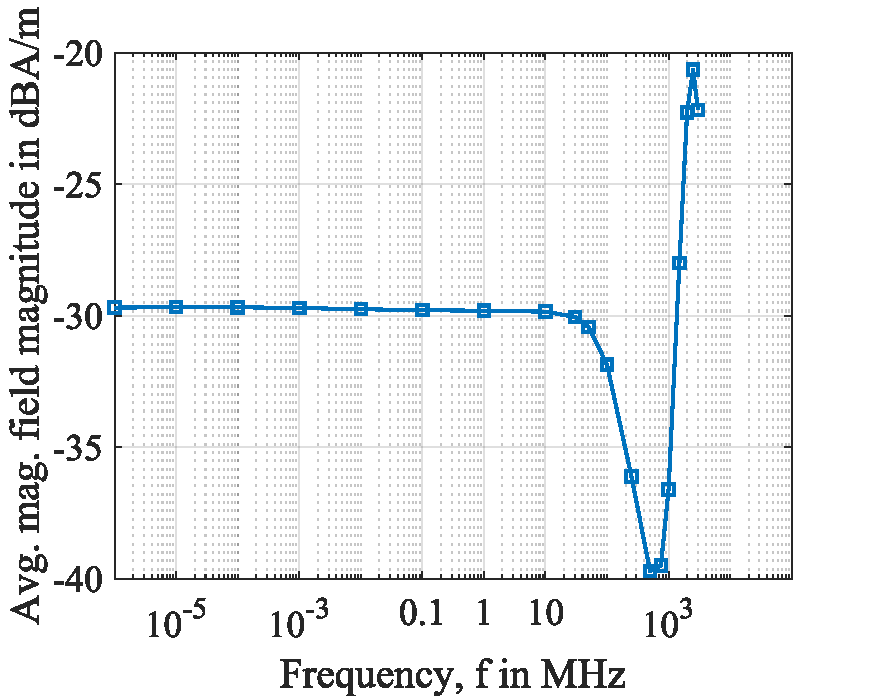
\includegraphics[width=0.32\textwidth]{loop_avh.pdf}&
				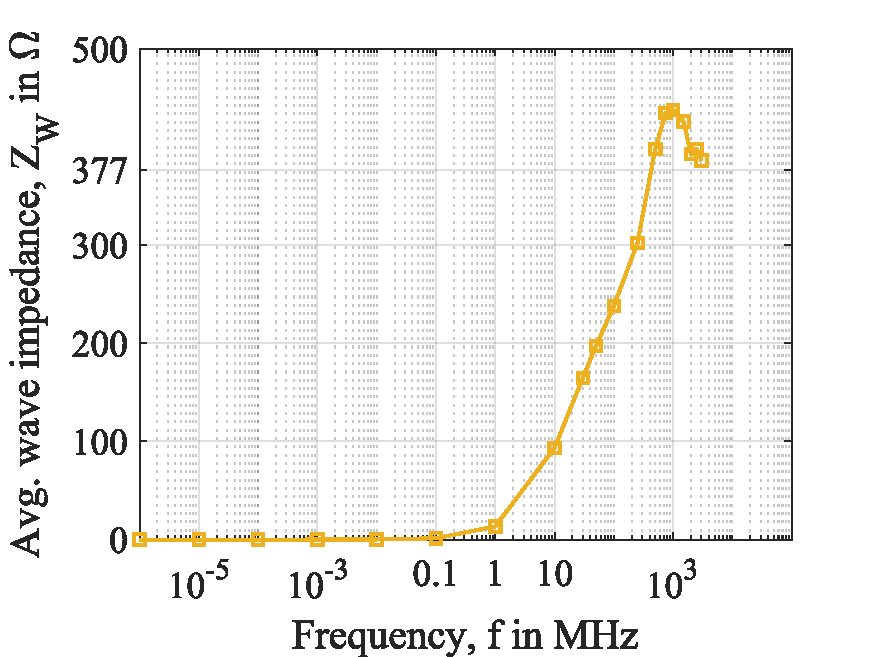
\includegraphics[width=0.32\textwidth]{loop_zw.pdf}
			\end{tabular}
		\end{figure}
		\column{0.2\textwidth}
		\vspace{3.2em}
		\captionof{figure}{Field magnitudes and wave impedance averaged in the sampling plane for the loop circuit.}
	\end{columns}
\end{frame}

\begin{frame}
	\frametitle{Patch Circuit}
	\begin{figure}
		\centering
		\begin{tabular}{ccc}
			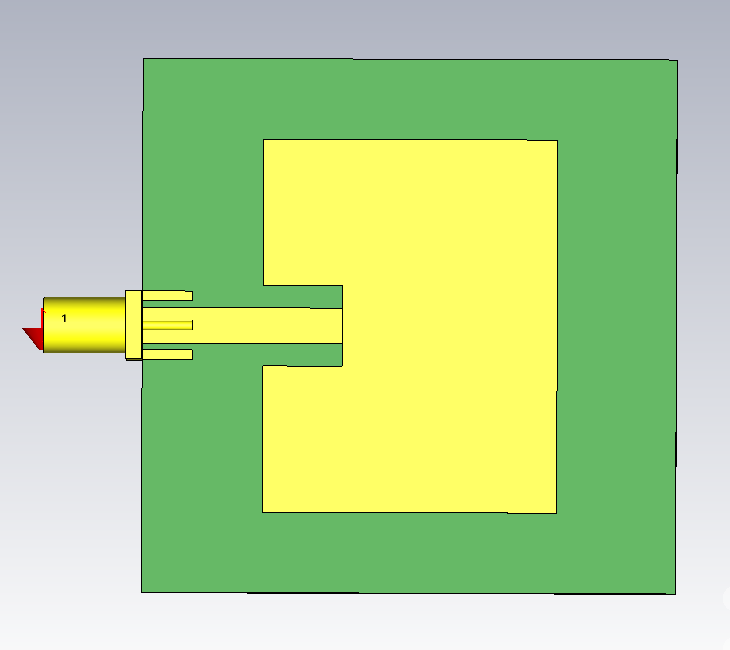
\includegraphics[width=0.25\textwidth]{patch.png}&
			\hspace{25pt}
			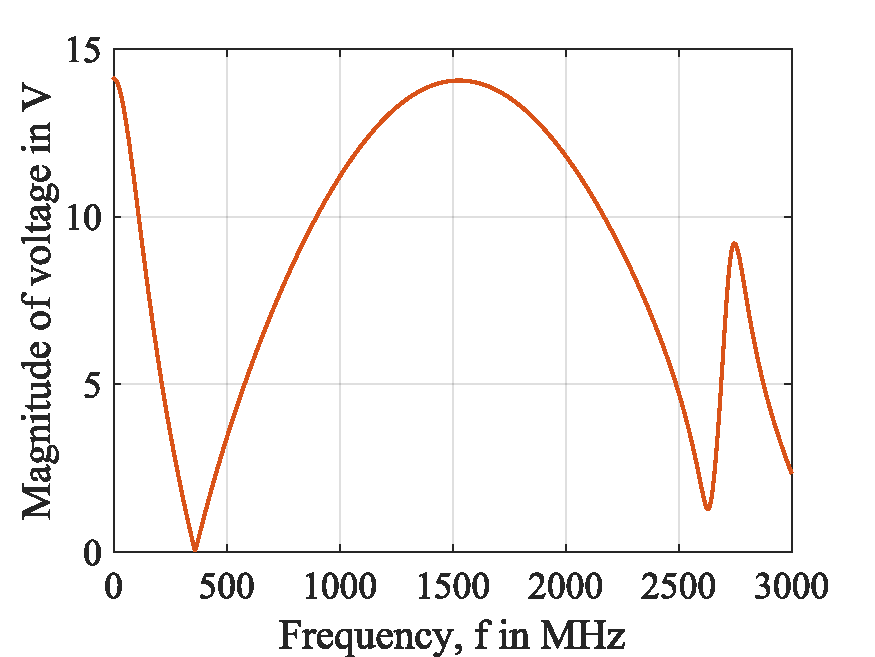
\includegraphics[width=0.3\textwidth]{patch_v.pdf}&
			\hspace{25pt}
			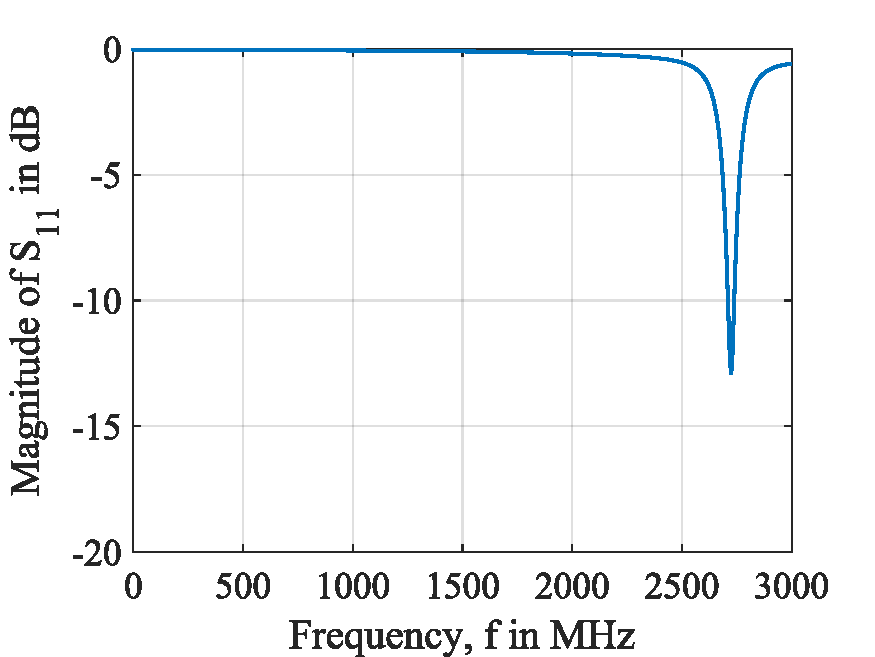
\includegraphics[width=0.3\textwidth]{patch_s11.pdf}
		\end{tabular}
		\caption{Patch circuit implemented in CST (left), the magnitude of voltage over it (middle) and magnitude of the $S_{11}$-parameter (right).}
	\end{figure}
	The circuit is implemented on a $\SI{50.8}{\milli\meter} \times \SI{50.8}{\milli\meter}$ Rogers RO4003C PCB with a ground plane at the bottom layer. The patch at the top layer has dimensions $\SI{28}{\milli\meter} \times \SI{35.5}{\milli\meter}$.
\end{frame}

\begin{frame}
	\frametitle{Patch Circuit}
	\begin{columns}
		\column{0.6\textwidth}
		\begin{figure}
			\centering
			\begin{tabular}{c}
				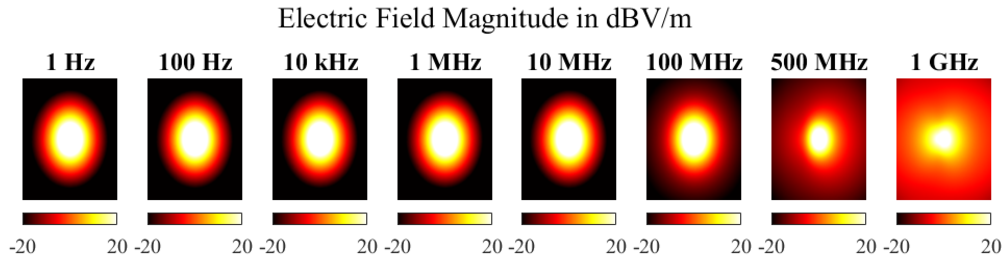
\includegraphics[width=\textwidth]{patch1.pdf}\\
				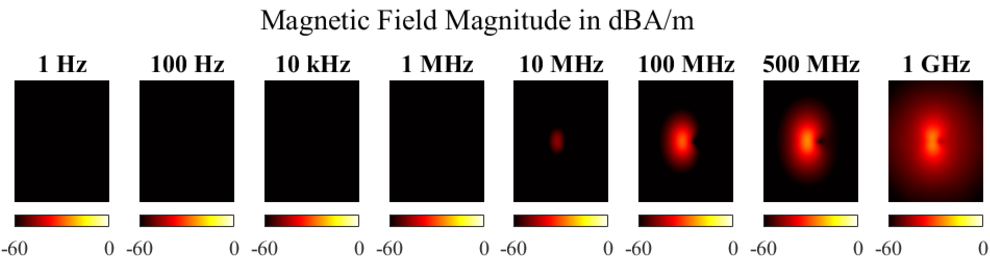
\includegraphics[width=\textwidth]{patch2.pdf}
			\end{tabular}
		\end{figure}
		\column{0.4\textwidth}
		\vspace{8em}
		\captionof{figure}{Near-field simulation results collected \SI{3}{\centi\meter} above the circuit in a $\SI{40}{\centi\meter} \times \SI{40}{\centi\meter}$ plane for the patch circuit.}
	\end{columns}
	\vspace{-20pt}
	\begin{columns}
		\column{0.8\textwidth}
		\begin{figure}
			\begin{tabular}{ccc}
				\includegraphics[width=0.32\textwidth]{patch_ave.pdf}&
				\includegraphics[width=0.32\textwidth]{patch_avh.pdf}&
				\includegraphics[width=0.32\textwidth]{patch_zw.pdf}
			\end{tabular}
		\end{figure}
		\column{0.2\textwidth}
		\vspace{3.2em}
		\captionof{figure}{Field magnitudes and wave impedance averaged in the sampling plane for the patch circuit.}
	\end{columns}
	
\end{frame}

\begin{frame}
	\frametitle{Coplanar Circuit}
	\begin{figure}
		\centering
		\begin{tabular}{ccc}
			\includegraphics[width=0.25\textwidth]{resistor.png}&
			\hspace{25pt}
			\includegraphics[width=0.3\textwidth]{resistor_v.pdf}&
			\hspace{25pt}
			\includegraphics[width=0.3\textwidth]{resistor_i.pdf}
		\end{tabular}
		\caption{Coplanar circuit implemented in CST (left), the magnitude of the voltage over it (middle) and magnitude of the current through (right).}
	\end{figure}
	The circuit is implemented on a $\SI{50.8}{\milli\meter} \times \SI{25.4}{\milli\meter}$ Rogers RO4003C PCB without a ground plane at the bottom layer.
\end{frame}

\begin{frame}
	\frametitle{Coplanar Circuit}
	\begin{columns}
		\column{0.6\textwidth}
		\begin{figure}
			\centering
			\begin{tabular}{c}
				\includegraphics[width=\textwidth]{resistor1.pdf}\\
				\includegraphics[width=\textwidth]{resistor2.pdf}
			\end{tabular}
		\end{figure}
		\column{0.4\textwidth}
		\vspace{8em}
		\captionof{figure}{Near-field simulation results collected \SI{3}{\centi\meter} above the circuit in a $\SI{40}{\centi\meter} \times \SI{40}{\centi\meter}$ plane for the resistor circuit.}
	\end{columns}
	\vspace{-20pt}
	\begin{columns}
		\column{0.8\textwidth}
		\begin{figure}
			\begin{tabular}{ccc}
				\includegraphics[width=0.32\textwidth]{resistor_ave.pdf}&
				\includegraphics[width=0.32\textwidth]{resistor_avh.pdf}&
				\includegraphics[width=0.32\textwidth]{resistor_zw.pdf}
			\end{tabular}
		\end{figure}
		\column{0.2\textwidth}
		\vspace{3.2em}
		\captionof{figure}{Field magnitudes and wave impedance averaged in the sampling plane for the resistor circuit.}
	\end{columns}
	
\end{frame}

\begin{frame}
	\frametitle{LC Bandpass Filters}
	\textbf{3rd order LC Bandpass filter, 1st variant}\\
	\vspace{-50pt}
	\begin{figure}
		\centering
		\begin{tabular}{ccc}
			\includegraphics[width=0.3\textwidth]{bpf.pdf}&
			\includegraphics[width=0.3\textwidth]{bpf.png}&
			\includegraphics[width=0.3\textwidth]{bpf_sparam.pdf}
		\end{tabular}
		\caption{Bandpass filter's circuit diagram (left), its implementation in CST (middle), and its important S-parameters.}
	\end{figure}
	\vspace{-20pt}
	The circuit is implemented on a $\SI{50.8}{\milli\meter} \times \SI{25.4}{\milli\meter}$ Rogers RO4003C PCB with a ground plane at the bottom layer.
	\vspace{-20pt}
	\begin{table}[ptbh]
		\centering
		\begin{tabular}{|c c c c c|}
			\hline
			$-$ & $L_1$ & $C_1$ & $L_2$ & $C_2$ \\
			\hline
			Component value & \SI{100}{\nano\henry} & \SI{1}{\nano\farad} & \SI{1.5}{\micro\henry} & \SI{68}{\pico\farad}\\
			Model number & 744912210 & 885342008003 & 7440450015 & 885342008010\\
			\hline
		\end{tabular} 
		\begin{tabular}{|c c c c|}
			\hline
			$-$ & $L_3$ & $C_3$ & $R_1$\\
			\hline
			Component value & \SI{100}{\nano\henry} & \SI{1}{\nano\farad} & \SI{50}{\ohm}\\
			Model number & 744912210 & 885342008003 & RCP1206W50R0GEB\\
			\hline
		\end{tabular}
		\caption{Obtained component values from design equations in \cite{lam} rounded to the closest standard value.}
	\end{table}
\end{frame}

\begin{frame}
	\frametitle{LC Bandpass Filters}
	\begin{columns}
		\column{0.6\textwidth}
		\begin{figure}
			\centering
			\begin{tabular}{c}
				\includegraphics[width=0.85\textwidth]{bpf1.pdf}\\
				\includegraphics[width=0.85\textwidth]{bpf2.pdf}
			\end{tabular}
				\caption{Near-field simulation results collected \SI{1}{\centi\meter} above the circuit in a $\SI{10}{\centi\meter} \times \SI{10}{\centi\meter}$ plane for the bandpass filter.}
		\end{figure}
		\column{0.4\textwidth}
		\vspace{1em}
		Reminder:
		\begin{figure}
			\centering
			\begin{tabular}{c}
				\includegraphics[width=0.7\textwidth]{bpf.pdf}\\
				\includegraphics[width=0.7\textwidth]{bpf.png}
			\end{tabular}
		\end{figure}
	\end{columns}
	\vspace{-35pt}
	\begin{columns}
		\column{0.8\textwidth}
		\begin{figure}
			\begin{tabular}{ccc}
				\includegraphics[width=0.32\textwidth]{bpf_ave.pdf}&
				\includegraphics[width=0.32\textwidth]{bpf_avh.pdf}&
				\includegraphics[width=0.32\textwidth]{bpf_zw.pdf}
			\end{tabular}
		\end{figure}
		\column{0.2\textwidth}
		\vspace{2.75em}
		\captionof{figure}{Average field magnitudes and wave impedance collected \SI{3}{\centi\meter} above the circuit in a $\SI{40}{\centi\meter} \times \SI{40}{\centi\meter}$ plane.}
	\end{columns}
	
\end{frame}

\begin{frame}
	\frametitle{LC Bandpass Filters}
	\textbf{3rd order LC Bandpass filter, 2nd variant}\\
	\vspace{-50pt}
	\begin{figure}
		\centering
		\begin{tabular}{ccc}
			\includegraphics[width=0.3\textwidth]{bpfs.pdf}&
			\includegraphics[width=0.3\textwidth]{bpfs.png}&
			\includegraphics[width=0.3\textwidth]{bpfs_sparam.pdf}
		\end{tabular}
		\caption{Circuit diagram (left), filter's implementation in CST (middle), and its important S-parameters.}
	\end{figure}
	\vspace{-20pt}
	The circuit is implemented on a $\SI{25.4}{\milli\meter} \times \SI{50.8}{\milli\meter}$ Rogers RO4003C PCB with a ground plane at the bottom layer.
	\vspace{-20pt}
	\begin{table}[ptbh]
		\centering
		\begin{tabular}{|c|c c c c|}
			\hline
			$-$ & $L_1$ & $C_1$ & $L_2$ & $C_2$ \\
			\hline
			Component value & \SI{1.5}{\micro\henry} & \SI{47}{\pico\farad} & \SI{100}{\nano\henry} & \SI{680}{\pico\farad}\\
			Model number & 7440450015 & 885342008001 & 744912210 & 885012007087\\
			\hline
		\end{tabular} 
		\begin{tabular}{|c|c c c|}
			\hline
			$-$ & $L_3$ & $C_3$ & $R_1$\\
			\hline
			Component value & \SI{1.5}{\micro\henry} & \SI{47}{\pico\farad} & \SI{50}{\ohm}\\
			Model number & 7440450015 & 885342008001 & RCP1206W50R0GEB\\
			\hline
		\end{tabular}
		\caption{Obtained component values from design equations in \cite{lam} rounded to the closest standard value.}
	\end{table}
\end{frame}

\begin{frame}
	\frametitle{LC Bandpass Filters}
	\begin{columns}
		\column{0.6\textwidth}
		\begin{figure}
			\centering
			\begin{tabular}{c}
				\includegraphics[width=0.85\textwidth]{bpfs1.pdf}\\
				\includegraphics[width=0.85\textwidth]{bpfs2.pdf}
			\end{tabular}
			\caption{Near-field simulation results collected \SI{1}{\centi\meter} above the circuit in a $\SI{10}{\centi\meter} \times \SI{10}{\centi\meter}$ plane for the bandpass filter second variant.}
		\end{figure}
		\column{0.4\textwidth}
		\vspace{1em}
		Reminder:
		\begin{figure}
			\centering
			\begin{tabular}{c}
				\includegraphics[width=0.7\textwidth]{bpfs.pdf}\\
				\includegraphics[width=0.7\textwidth]{bpfs.png}
			\end{tabular}
		\end{figure}
	\end{columns}
	\vspace{-40pt}
	\begin{columns}
		\column{0.8\textwidth}
		\begin{figure}
			\begin{tabular}{ccc}
				\includegraphics[width=0.32\textwidth]{bpfs_ave.pdf}&
				\includegraphics[width=0.32\textwidth]{bpfs_avh.pdf}&
				\includegraphics[width=0.32\textwidth]{bpfs_zw.pdf}
			\end{tabular}
		\end{figure}
		\column{0.2\textwidth}
		\vspace{2.75em}
		\captionof{figure}{Average field magnitudes and wave impedance collected \SI{3}{\centi\meter} above the circuit in a $\SI{40}{\centi\meter} \times \SI{40}{\centi\meter}$ plane.}
	\end{columns}
	
\end{frame}

\begin{frame}
	\frametitle{Lumped Wilkinson Divider}
	%\vspace{-50pt}
	\begin{figure}
		\centering
		\begin{tabular}{cc}
			\includegraphics[width=0.3\textwidth]{wilkinson_dist.pdf}&
			\includegraphics[width=0.35\textwidth]{wilkinson.pdf}\\
			\includegraphics[width=0.3\textwidth]{wilkinson.png}&
			\includegraphics[width=0.25\textwidth]{wilkinson_sparam.pdf}
		\end{tabular}
		\caption{Distributed implementation (top-left), lumped implementation (top-right). Implemented lumped Wilkinson divider in CST (bottom-left) and its important S-parameters (bottom-right).}
	\end{figure}
	\vspace{-20pt}
	$L = Z_0/\omega_0$ and $C = 1/(Z_0\omega_0)$\cite{9422969}\\
	For this circuit, $Z_0 = \SI{50}{\ohm}$, $L = \SI{2.2}{\micro\henry}$ and $C = \SI{440}{\pico\farad}$, thus $L_1 = L_2 =  \SI{2.2}{\micro\henry}$, $C_2 = C_3 = \SI{440}{\pico\farad}$, $C_1 = \SI{1}{\nano\farad}$, after rounding to the closest standard values.
\end{frame}

\begin{frame}
	\frametitle{Lumped Wilkinson Divider}
	\begin{columns}
		\column{0.6\textwidth}
		\begin{figure}
			\centering
			\begin{tabular}{c}
				\includegraphics[width=0.85\textwidth]{wilkinson1.pdf}\\
				\includegraphics[width=0.85\textwidth]{wilkinson2.pdf}
			\end{tabular}
			\caption{Near-field simulation results collected \SI{1}{\centi\meter} above the circuit in a $\SI{10}{\centi\meter} \times \SI{10}{\centi\meter}$ plane for the Wilkinson divider.}
		\end{figure}
		\column{0.4\textwidth}
		\vspace{1em}
		Reminder:
		\begin{figure}
			\centering
			\begin{tabular}{c}
				\includegraphics[width=0.7\textwidth]{wilkinson.pdf}\\
				\includegraphics[width=0.7\textwidth]{wilkinson.png}
			\end{tabular}
		\end{figure}
	\end{columns}
	\vspace{-35pt}
	\begin{columns}
		\column{0.8\textwidth}
		\begin{figure}
			\begin{tabular}{ccc}
				\includegraphics[width=0.32\textwidth]{wilkinson_ave.pdf}&
				\includegraphics[width=0.32\textwidth]{wilkinson_avh.pdf}&
				\includegraphics[width=0.32\textwidth]{wilkinson_zw.pdf}
			\end{tabular}
		\end{figure}
		\column{0.2\textwidth}
		\vspace{2.5em}
		\captionof{figure}{Average field magnitudes and wave impedance collected \SI{3}{\centi\meter} above the circuit in a $\SI{40}{\centi\meter} \times \SI{40}{\centi\meter}$ plane.}
	\end{columns}
	
\end{frame}

\begin{frame}{Conclusion} 
In this work the design and implementation of various test circuits with different near-field patterns in CST to test an inverse source solver at low frequencies. 

In the first part of the work, the theory of SMD components that are used to implement some of these circuits was presented which includes drum core inductors, air core inductors, multilayer ceramic capacitors and chip resistor.

In the second part of the work the test circuits are implemented which include loop circuits with dominant magnetic field at low frequencies, microstrip circuits with dominant electric field at low frequencies, and the coplanar circuit that has both fields at low frequencies. In addition, basic resonant circuits including bandpass filters, Wilkinson dividers, and hybrid couplers, are implemented of which two bandpass filters and one divider is examined in detail.
\end{frame}

\begin{frame}[c, allowframebreaks]{References} 
	\printbibliography
\end{frame}

%%%%%%%%%%%%%%%%%%%%%%%%%%%%%%%%%%%%%%%%%%%%%%%%%%%%%%%%%%%%%%%%%%%%%%%%%%%%%%%%
\end{document} % !!! NICHT ENTFERNEN !!!
%%%%%%%%%%%%%%%%%%%%%%%%%%%%%%%%%%%%%%%%%%%%%%%%%%%%%%%%%%%%%%%%%%%%%%%%%%%%%%%%

